%%%%%%%%%%%%%%%%%%%%%%% file template.tex %%%%%%%%%%%%%%%%%%%%%%%%%
%
% This is a general template file for the LaTeX package SVJour3
% for Springer journals.          Springer Heidelberg 2010/09/16
%
% Copy it to a new file with a new name and use it as the basis
% for your article. Delete % signs as needed.
%
% This template includes a few options for different layouts and
% content for various journals. Please consult a previous issue of
% your journal as needed.
%
%%%%%%%%%%%%%%%%%%%%%%%%%%%%%%%%%%%%%%%%%%%%%%%%%%%%%%%%%%%%%%%%%%%
%
% First comes an example EPS file -- just ignore it and
% proceed on the \documentclass line
% your LaTeX will extract the file if required
\begin{filecontents*}{example.eps}
%!PS-Adobe-3.0 EPSF-3.0
%%BoundingBox: 19 19 221 221
%%CreationDate: Mon Sep 29 1997
%%Creator: programmed by hand (JK)
%%EndComments
gsave
newpath
  20 20 moveto
  20 220 lineto
  220 220 lineto
  220 20 lineto
closepath
2 setlinewidth
gsave
  .4 setgray fill
grestore
stroke
grestore
\end{filecontents*}
%
\RequirePackage{fix-cm}
%
\documentclass[twocolumn]{svjour3}         % twocolumn
%\documentclass[smallcondensed]{svjour3}     % onecolumn (ditto)
%\documentclass[smallextended]{svjour3}       % onecolumn (second format)
%\documentclass{svjour3}                     % onecolumn (standard format)
%
\smartqed  % flush right qed marks, e.g. at end of proof
%
%
% \usepackage{mathptmx}      % use Times fonts if available on your TeX system
%
% insert here the call for the packages your document requires
\usepackage{graphicx}
\graphicspath{{../}{./}}
\usepackage{booktabs}
\usepackage{amsmath}
\usepackage{hyperref}
\usepackage{array}
\usepackage{enumitem}
\usepackage{microtype}
\usepackage{xspace}
\usepackage{CJKutf8}

\emergencystretch=1.5em

\newcommand{\algname}{ReRAPTOR\xspace}
%\usepackage{latexsym}
% etc.
%
% please place your own definitions here and don't use \def but
% \newcommand{}{}
%
% Insert the name of "your journal" with
% \journalname{myjournal}
%
\begin{document}

\title{ReRAPTOR: Reverse-Objective RAPTOR for Time-Budgeted Value-Maximizing Transit Itinerary Planning}
%\subtitle{Subtitle}

\titlerunning{ReRAPTOR for Value-Maximizing Transit Itinerary Planning}

\author{Bin Zhou \and
    Guangxian Li \and
    Teruki Ogo \and
    Yutaka Arakawa \and
    Tsunenori Mine %etc.
}

%\authorrunning{Short form of author list} % if too long for running head

\institute{Bin Zhou \at
    Graduate School of Information Science and Electrical Engineering, Kyushu University, Fukuoka, Japan \\
    \email{zhou.bin.883@s.kyushu-u.ac.jp}
    \and
    Guangxian Li \at
    Graduate School of Information Science and Electrical Engineering, Kyushu University, Fukuoka, Japan \\
    \email{li.guangxian.021@s.kyushu-u.ac.jp}
    \and
    Teruki Ogo \at
    Faculty of Information Science and Engineering, Kyushu Sangyo University, Fukuoka, Japan \\
    \email{k25rm021@st.kyusan-u.ac.jp}
    \and
    Yutaka Arakawa \at
    Faculty of Information Science and Electrical Engineering, Kyushu University, Fukuoka, Japan \\
    \email{arakawa@ait.kyushu-u.ac.jp}
    \and
    Tsunenori Mine \at
    Faculty of Information Science and Electrical Engineering, Kyushu University, Fukuoka, Japan \\
    \email{mine@ait.kyushu-u.ac.jp}
}

\date{Received: date / Accepted: date}
% The correct dates will be entered by the editor


\maketitle

\begin{abstract}
    Public-transit routing is usually formulated as an earliest-arrival problem,
    but leisure exploration and time-budgeted outing design require
    timetable-feasible routes that maximize itinerary value rather than merely
    minimize travel time. This paper studies time-budgeted value-maximizing
    transit itinerary planning on timetable-based transit schedules and proposes ReRAP\-TOR, a
    reverse-objective RAPTOR-style label-setting method that preserves
    timetable-feasible expansion while ranking partial routes by a value-aware
    surrogate score. The framework supports pluggable objective modules and uses
    three pruning layers: Beam pruning for width control, Dominance pruning for
    local label filtering, and Negative pruning for suppressing semantically
    weak partial routes. We evaluate the method on Ekispert-provided transit
    schedule data for Fukuoka under a seeded stop-reward benchmark and compare
    it with
    NSGA-II, ILS+2opt, VNS, SA, McRAPTOR, Pure RAPTOR, and Greedy.
    ReRAPTOR achieves the
    highest overall average stop score (\(826.90\)), improving on
    NSGA-II by
    \(8.71\%\), while remaining \(6.57\times\) faster on average
    (\(4165.67\) ms vs \(27351.18\) ms). A supplementary balance analysis
    further shows that ReRAPTOR is the closest method to the score--time ideal
    point, with query-level ideal distance \(0.1672\) versus \(0.6292\) for
    NSGA-II. Ablation results show that Beam and Dominance are the two core
    scalability layers, whereas Negative pruning mainly improves semantic
    alignment in theme-constrained tasks. These results indicate that ReRAPTOR
    provides a strong quality--speed trade-off for value-oriented transit
    itinerary planning.
    \keywords{Transit itinerary planning \and Transit schedule data \and RAPTOR \and Time-budgeted route planning \and Multi-objective search}
    % \PACS{PACS code1 \and PACS code2 \and more}
    % \subclass{MSC code1 \and MSC code2 \and more}
\end{abstract}

\section{Introduction}
Public-transit route planning is traditionally formulated as a timetable-feasible
earliest-arrival problem \cite{agarwal2024bicriteriontb,delling2019restrictedpareto,delling2015raptor,he2022paretojourneys}.
That formulation is appropriate for commuters, but it does not capture the needs
of leisure travelers, city explorers, or users who want to spend a fixed amount
of time on transit while collecting as much route value as possible.
In these settings, a good itinerary is not defined only by arrival time.
It may also depend on ride duration, the number of distinct stops visited,
spatial spread, and the thematic or semantic quality of the route.
The problem is therefore closer to time-budgeted itinerary design than to
classical shortest-path search \cite{gunawan2016survey,ruizmeza2022slr,souffriau2008personalized}.

\begin{figure*}[t]
    \centering
    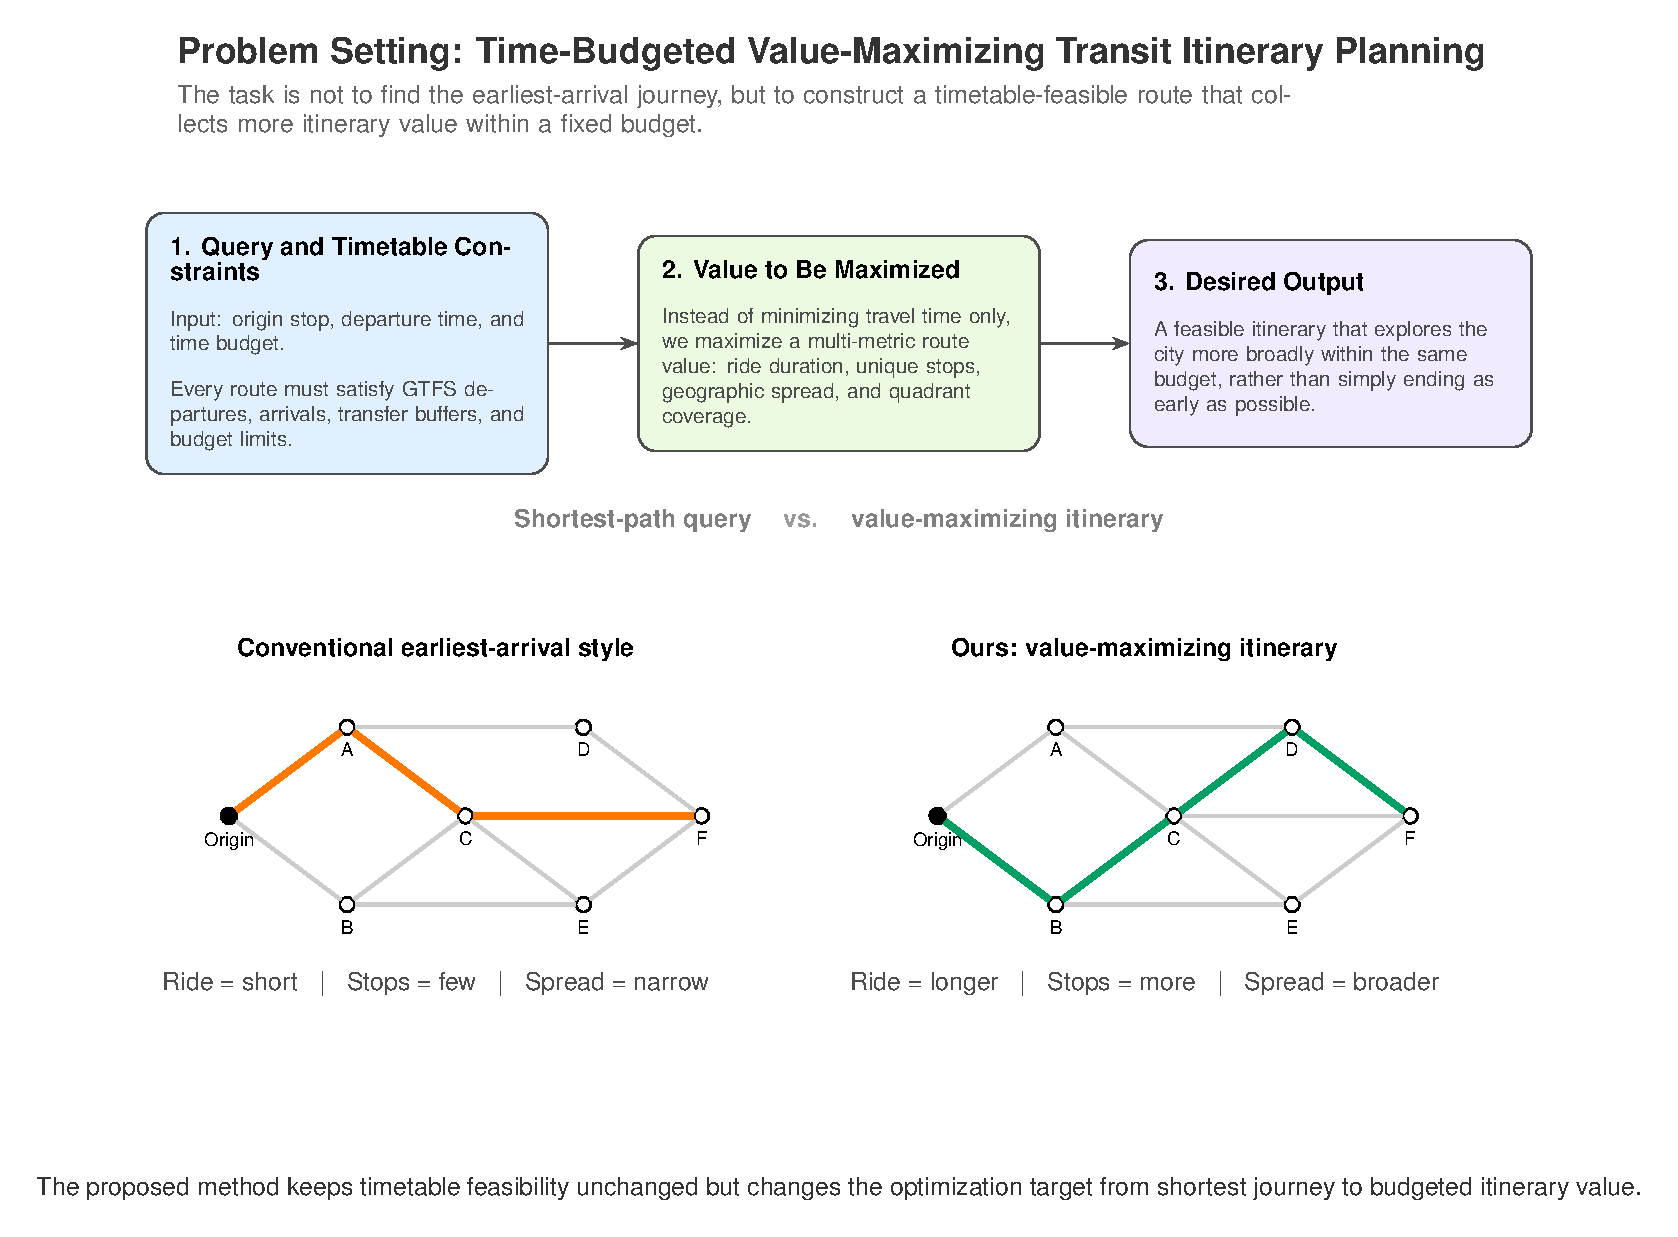
\includegraphics[width=0.94\textwidth]{figures/method/intro_problem_overview.pdf}
    \caption{Problem overview of time-budgeted value-maximizing transit itinerary planning. Unlike conventional earliest-arrival routing, the goal is to keep timetable feasibility while maximizing multi-dimensional itinerary value within a fixed travel budget.}
    \label{fig:intro_problem_overview}
\end{figure*}

The main technical difficulty is the combination of timetable feasibility and
value-oriented search.
Every candidate route must respect scheduled departures, arrivals, and transfer
constraints, while the search objective depends on accumulated route structure
rather than on arrival time alone.
Once stop diversity, spatial expansion, revisit patterns, or task-specific stop
rewards are incorporated, the number of plausible partial routes grows quickly.
An overly aggressive compression strategy removes information needed for value
maximization, whereas an unpruned search becomes computationally unstable.

This paper addresses that gap with ReRAP\-TOR, a reverse-objective RAPTOR-style
search over timetable-feasible transit stop schedules \cite{delling2015raptor,wessel2017retrospective,wong2013leveraginggtfs}.
Instead of propagating labels to minimize arrival time, ReRAPTOR preserves the
timetable-feasible expansion logic of RAPTOR while ranking partial routes by a
task-dependent value surrogate.
The framework is generic: the search backbone is shared, while the scoring and
acceptance modules can be instantiated for geometry-aware exploration or for the
seeded stop-reward task used in our main experiments.
To keep the search tractable, ReRAPTOR combines three pruning layers: Beam
pruning for width control, Dominance pruning for local label filtering, and
Negative pruning for rejecting semantically weak or clearly low-quality partial
routes.
Figure~\ref{fig:intro_problem_overview} illustrates this shift from
earliest-arrival routing to time-budgeted value collection.

We evaluate the method on Ekispert-provided transit schedule data for Fukuoka
through four experiment groups.
Experiment~1 compares ReRAPTOR with NSGA-II~\cite{deb2002nsga2},
ILS+2opt~\cite{lourenco2003ils}, VNS~\cite{mladenovic1997vns},
SA~\cite{kirkpatrick1983sa}, McRAPTOR and Pure RAPTOR~\cite{delling2015raptor},
and Greedy under a seeded stop-reward benchmark.
ReRAPTOR achieves the highest overall average stop score (\(826.90\)) and is
\(6.57\times\) faster than NSGA-II on average (\(4165.67\) ms vs
\(27351.18\) ms).
Experiment~2 shows that Beam and Dominance are the two core scalability layers:
removing Dominance makes the method \(2.91\times\) slower, removing Beam makes
it \(9.53\times\) slower, and removing both causes severe label explosion and
cap hits.
Experiment~3 further shows that ReRAPTOR is the closest method to the
score--time ideal point, with query-level ideal distance \(0.1672\) compared
with \(0.6292\) for NSGA-II.
Experiment~4 complements the aggregate numbers with route-level cases, including
both strong success cases and an explicit counterexample.

The contributions of this paper are fourfold.
First, we formulate time-budgeted value-maximizing transit itinerary planning
as a timetable-feasible search problem with pluggable objective and acceptance
modules, so the same search backbone can support geometry-aware and seeded
stop-reward tasks.
Second, we propose ReRAP\-TOR, a reverse-objective RAPTOR-style label-setting
algorithm that keeps route history, spatial coverage, and task-specific reward
state inside timetable expansion rather than scoring routes only after
construction.
Third, we show that the proposed three-layer pruning design has distinct roles:
Beam and Dominance act as the main search-space control layers, whereas
Negative pruning mainly improves semantic alignment in constrained tasks.
Fourth, experiments on Ekispert-provided Fukuoka transit schedules show that
ReRAPTOR achieves the strongest overall quality--speed profile among the
compared baselines while remaining explicit about failure cases.

The remainder of the paper is organized as follows.
Section 2 reviews related work on tourist trip design, public-transit routing,
and multi-objective search.
Section 3 formalizes the problem.
Section 4 presents ReRAPTOR and its mathematical abstraction.
Section 5 reports experimental results, including algorithm comparison, ablation, balance analysis,
and a route case study.
Finally, Sections 6 and 7 discuss implications and conclude the paper.

\section{Related Work}
Timetable-based public-transit routing has been studied extensively, with RAPTOR
being a representative round-based framework for computing efficient
earliest-arrival and Pareto-feasible journeys without heavy preprocessing
\cite{delling2015raptor}. Subsequent work improves exact or near-exact search
through trip-based bicriterion routing, transfer-aware Pareto exploration,
restricted Pareto sets, hyper-partitioning, hub-label acceleration, and transfer
connection databases
\cite{abuaisha2024transferdb,agarwal2024bicriteriontb,delling2019restrictedpareto,delling2017hyperpartitioning,he2022paretojourneys,phan2019hublabeling}.
Other studies consider public-transport routing objectives beyond travel time,
including fare or price optimization and multi-objective Monte-Carlo tree search
\cite{euler2024price,weng2021mcts}. However, these methods mainly target
earliest-arrival, transfer-minimizing, fare-aware, or Pareto-routing queries,
rather than itinerary design under a fixed budget where route value depends on
accumulated route structure and exploration history.

GTFS has also become a common substrate for public-transport analysis and
algorithm design. Prior work has used GTFS for efficient transit analysis,
retrospective timetable reconstruction, time-geographic analysis, and database
querying of public-transport networks
\cite{godfrid2022mobilitydb,pereira2022gtfs2gps,wessel2017retrospective,wong2013leveraginggtfs}.
Public transport network datasets have further been assembled to support
algorithmic evaluation across cities \cite{kujala2018datasets}. These studies
show that GTFS is a practical and reproducible data source, but they do not
directly address value-maximizing itinerary search on timetable-feasible stop
schedules.

The itinerary-design side of our problem is closely related to the tourist trip
design problem and the broader orienteering family. Surveys show that
budget-constrained profit collection, team orienteering, time windows, and
preference-aware route construction are central themes in this literature
\cite{gunawan2016survey,ruizmeza2022slr}. Representative works study
personalized tourist trip design, trip-planning functionalities, time-dependent
team orienteering for tourist routing, and social-sensing-based personalization
\cite{gavalas2015teamorienteering,persia2020socialsensing,pilato2023modular,souffriau2010functionalities,souffriau2008personalized}.
Recent variants further consider green or fuzzy objectives, hotel selection,
capacity constraints, mandatory visits, GRASP-based multimodal optimization, and
incremental local search
\cite{ataei2022hotel,divsalar2022green,gonzaleznavasa2023transporttime,isik2024cp,luo2022capacity,marzal2024incrementalls,ruizmeza2021grasp,ruizmeza2022greenfuzzy,sylejmani2024patterns}.
Despite their richness, these formulations often assume free movement between
points of interest or simplified travel-time models, rather than operating
directly on timetable-feasible transit stop schedules.

More generally, multi-objective trip planning and shortest-path research has
studied ranking, preference integration, and dominance filtering in route
search \cite{choachaicharoenkul2022tripplanning,demeyer2013martins,fan2009urbanrouting,tenemaza2020itinerary}.
On the optimization side, canonical general-purpose baselines for value-guided
search include NSGA-II, iterated local search, variable neighborhood search,
and simulated annealing
\cite{deb2002nsga2,kirkpatrick1983sa,lourenco2003ils,mladenovic1997vns}.
Our work differs from both classical public-transit routing and tourist-trip
design in one specific way: it embeds a pluggable value module inside a
RAPTOR-style timetable search, so that itinerary value is optimized during
feasible schedule expansion rather than only after constructing a route.

\section{Problem Formulation}
We model the transit timetable as a temporal directed graph
\cite{pereira2022gtfs2gps,wessel2017retrospective,wong2013leveraginggtfs}
\(G=(\mathcal{S},\mathcal{E})\), where each stop \(s \in \mathcal{S}\) is a station
identifier and each edge \(e \in \mathcal{E}\) is a feasible timetable segment
\(e=(u,v,\tau^{\mathrm{dep}}(e),\tau^{\mathrm{arr}}(e),\ell(e),d(e))\).
Here \(u\) and \(v\) are origin and destination stops,
\(\tau^{\mathrm{dep}}\) and \(\tau^{\mathrm{arr}}\) are departure/arrival times,
\(\ell(e)\) is the transit line ID, and \(d(e)\) is the segment distance.
Given a query \(q=(o,t_0,B)\) with origin \(o\), departure time \(t_0\), and
time budget \(B\), the task is to construct a timetable-feasible itinerary
\(r=(e_1,\ldots,e_m)\) that maximizes route value.

A route is feasible if it starts from the query origin, respects stop continuity,
satisfies transfer-buffer constraints, and finishes within the budget:
\begin{equation}
    \label{eq:feasibility}
    \begin{aligned}
        u(e_1)                   & = o,                                                \\
        \tau^{\mathrm{dep}}(e_1) & \ge t_0,                                            \\
        v(e_i)                   & = u(e_{i+1}),                                       \\
        \tau^{\mathrm{dep}}(e_{i+1})
                                 & \ge \tau^{\mathrm{arr}}(e_i) + \delta(e_i,e_{i+1}), \\
        \tau^{\mathrm{arr}}(e_m) & \le t_0 + B,
    \end{aligned}
\end{equation}
where \(\delta(e_i,e_{i+1})=0\) for same-trip continuation and
\(\delta(e_i,e_{i+1})=\Delta_{\mathrm{tr}}\) otherwise.

Instead of fixing one route-value function for all tasks, we define a generic
objective module parameterized by \(\theta\):
\begin{equation}
    \label{eq:generic_objective}
    \max_{r \in \mathcal{R}(q)} \; F_{\theta}(r)
    \qquad
    \text{s.t. }
    g_{\theta}(r)=1,
\end{equation}
where \(\mathcal{R}(q)\) is the set of timetable-feasible routes under
Eq.~\ref{eq:feasibility}, \(F_{\theta}\) is a scenario-specific route-value
function, and \(g_{\theta}\) is an optional acceptance predicate. This
separation is important in our setting because the search backbone remains
unchanged across experiments, while only the value module and acceptance logic
are instantiated differently.

The default geometry-aware instance in the original formulation evaluates four
positive criteria:
\(f_1(r)\) = ride duration,
\(f_2(r)\) = number of unique visited stops,
\(f_3(r)\) = convex-hull area of visited stop coordinates, and
\(f_4(r)\) = quadrant coverage around the city center.
Using normalizers \(c_1=480\), \(c_2=50\), \(c_3=100\), and \(c_4=4\), we define
\(\tilde{f}_j(r)=f_j(r)/c_j\) and optimize
\begin{equation}
    \label{eq:objective_geometry}
    F_{\mathrm{geo}}(r) = \sum_{j=1}^{4} \alpha_j \tilde{f}_j(r),
\end{equation}
The default weights are \(0.40\), \(0.25\), \(0.20\), and \(0.15\).
Here \(c_1=480\) and \(c_4=4\) come from the problem itself:
the 8-hour budget ceiling and the maximum of four covered quadrants.
By contrast, \(c_2=50\) and \(c_3=100\) are reference scales that keep the
stop-count and hull-area terms comparable.
The weight vector is not re-tuned in this paper.
We keep the balanced geometry-aware profile from the original Fukuoka system,
with ride duration as the main term, stop diversity as the second term,
and spatial spread as supporting evidence.

Experiments~1--3 use a seeded stop-reward instantiation. Each stop
\(s \in \mathcal{S}\) receives a reward \(w_{\omega}(s)\) drawn once from a
random seed \(\omega\), and each unique non-origin stop incurs a dwell time
\(\eta\). Let \(V^{+}(r)\) denote the set of unique visited stops excluding the
origin, and let \(T(r)\) be the elapsed timetable travel time of route \(r\).
The effective task time is
\begin{equation}
    \label{eq:effective_time}
    T_{\eta}(r) = T(r) + \eta \, |V^{+}(r)|.
\end{equation}
The seeded stop-reward objective is then
\begin{equation}
    \label{eq:objective_stop_reward}
    F_{\omega,\eta}(r) = \sum_{s \in V^{+}(r)} w_{\omega}(s),
    \qquad
    g_{\omega,\eta}(r)=\mathbf{1}\!\left[T_{\eta}(r)\le B\right].
\end{equation}
In other words, the main experiments no longer optimize hull area directly;
they optimize collected stop reward under a fixed effective-time budget, while
the same timetable-feasible search structure and pruning framework are retained.

\section{Proposed Method}
\subsection{Overall Framework}
ReRAPTOR is a RAPTOR-style label-setting search over timetable-feasible transit stop schedules with
pluggable objective modules and a three-layer pruning mechanism
\cite{delling2015raptor,he2022paretojourneys}.
Unlike earliest-arrival transit routing, the search state explicitly stores
route history and exploration statistics. Partial itineraries can therefore be
ranked by both budgeted utility and route structure.
At a high level, the framework has five stages:
\begin{enumerate}[leftmargin=1.5em]
    \item load transit stop schedules and query parameters;
    \item initialize a base label at the origin stop;
    \item iteratively expand timetable-feasible outgoing edges from marked stops;
    \item evaluate each new partial itinerary with an objective-specific surrogate score and prune it with the three-layer filter;
    \item return the highest-scored accepted label as the final route.
\end{enumerate}

\begin{figure*}[t]
    \centering
    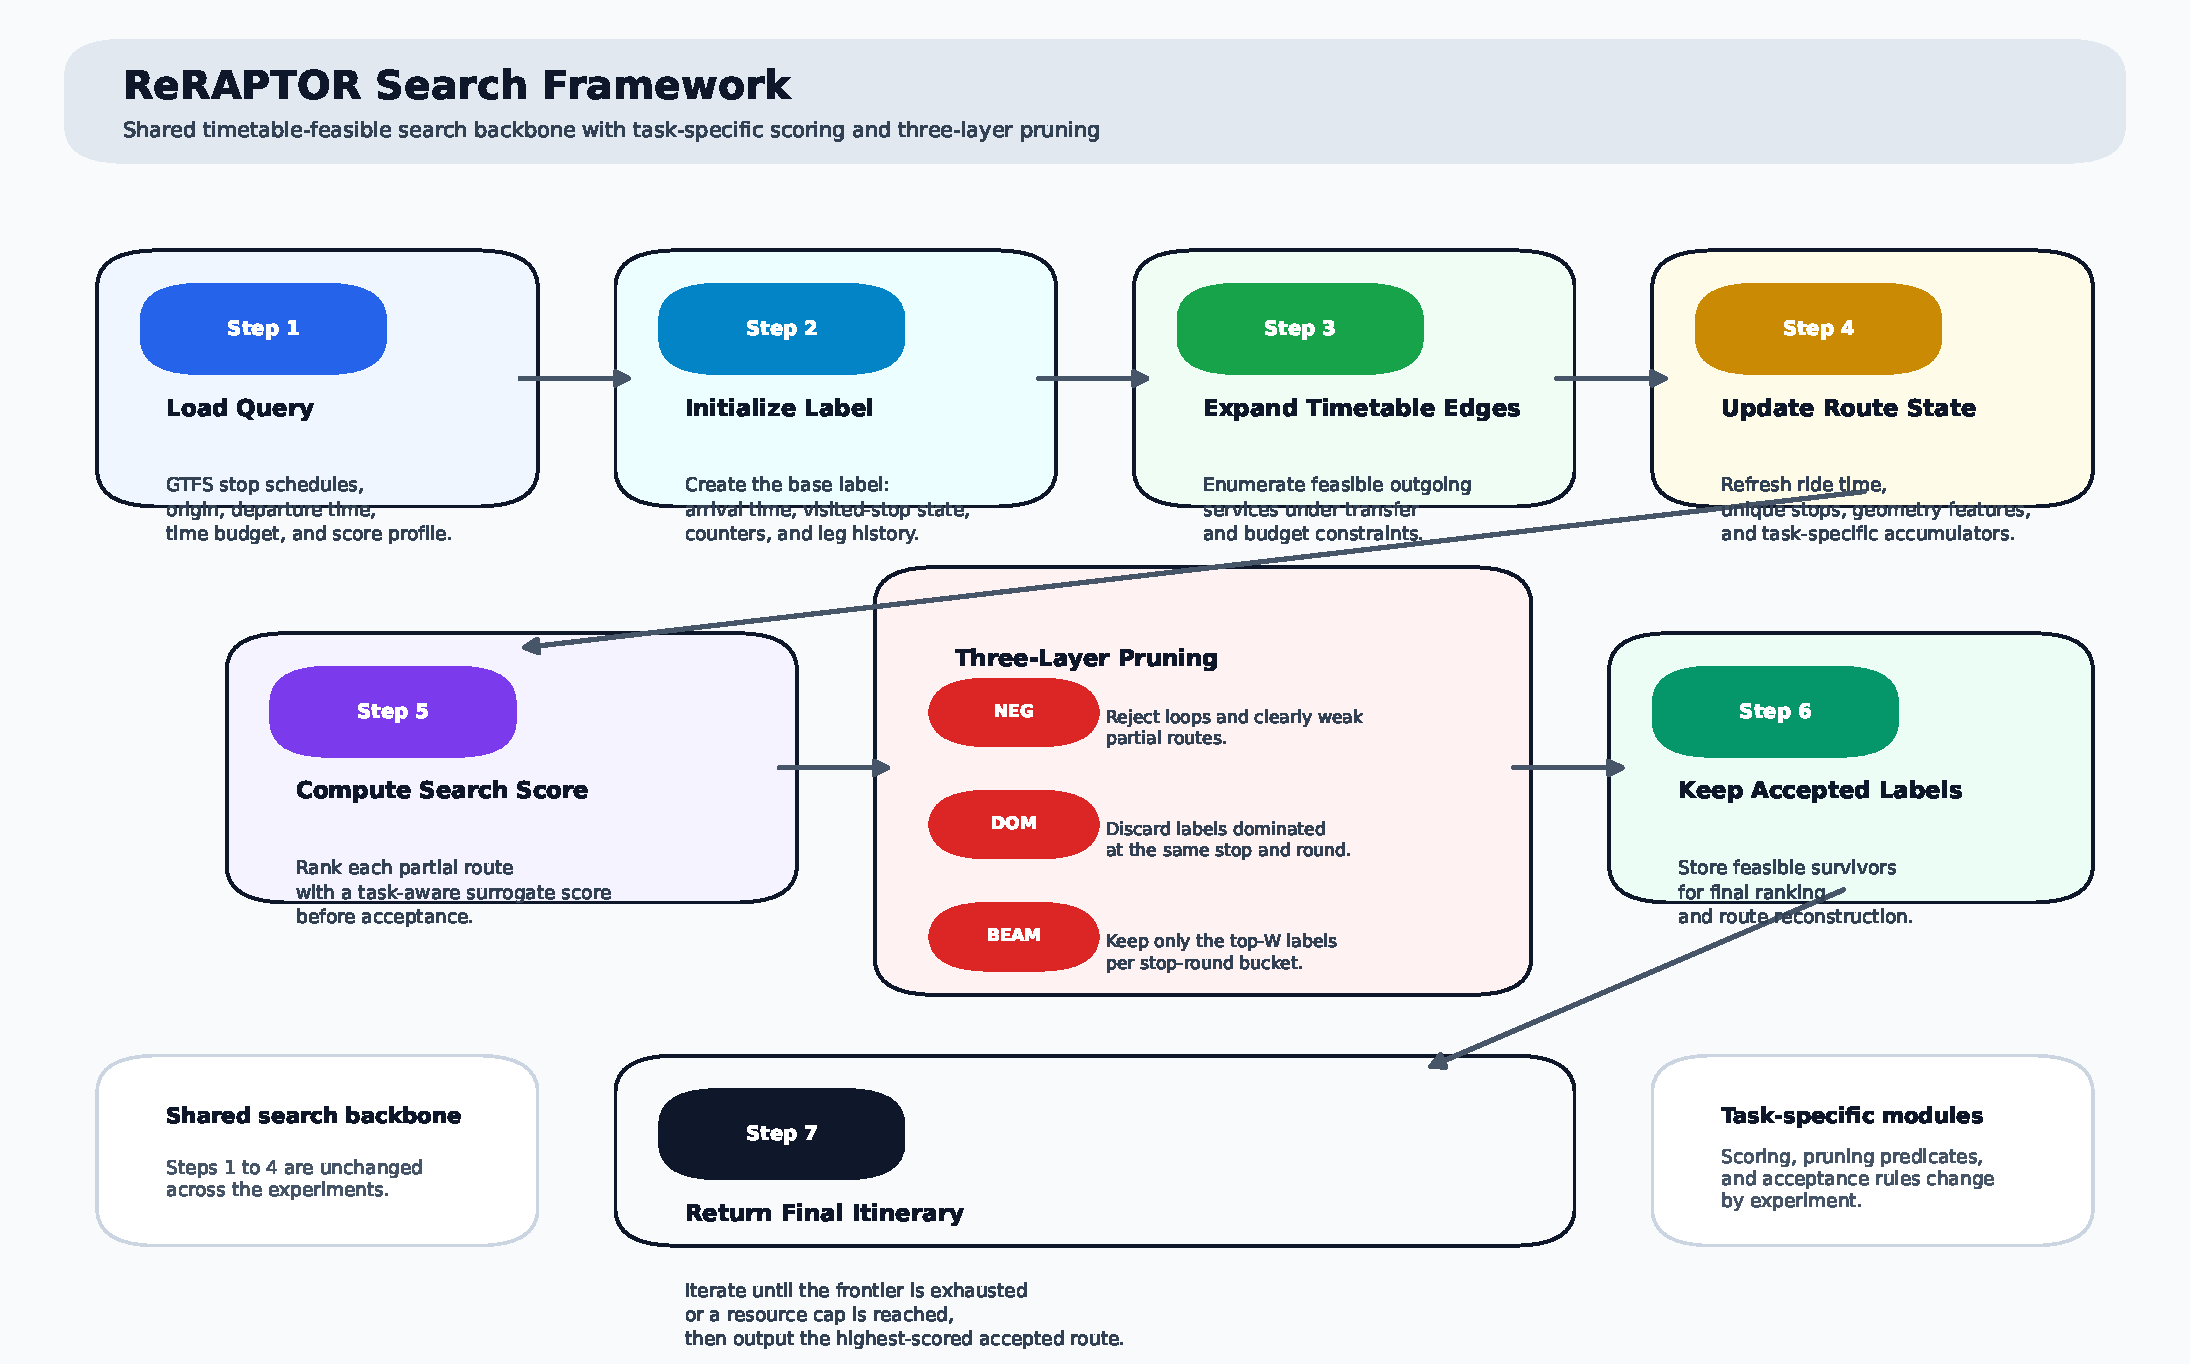
\includegraphics[width=0.94\textwidth]{figures/method/ours_framework_flow.pdf}
    \caption{Overall framework of the proposed time-budgeted itinerary planner. The core search remains unchanged across experiments; only score weights or optional acceptance predicates are varied.}
    \label{fig:method_framework}
\end{figure*}

Figure~\ref{fig:method_framework} highlights the separation between the shared
search backbone and the pluggable scoring/acceptance modules.
This separation lets us study algorithmic comparison (Exp1), pruning effects
(Exp2), and balance behavior (Exp3) without redesigning the search engine.

\subsection{Core Algorithm}
Each partial route is represented by a label
\begin{equation}
    \label{eq:label}
    \lambda =
    \left(
    a,\rho,d,V,q,\Pi,
    c^{\mathrm{stop}},c^{\mathrm{line}},
    n^{\mathrm{tr}},\psi
    \right),
\end{equation}
where \(a\) is the current arrival time, \(\rho\) is accumulated ride time,
\(d\) is traveled distance, \(V\) is the set of visited stops, \(q\) is a
bit-mask encoding covered quadrants, \(\Pi\) is the ordered leg sequence,
\(c^{\mathrm{stop}}\) and \(c^{\mathrm{line}}\) are visit counters, and
\(n^{\mathrm{tr}}\) is the number of transfers. The additional term
\(\psi\) stores objective-specific accumulators. In the stop-reward task used
for Experiments~1--3, \(\psi\) includes at least the collected reward total
\(\sigma\) and the number of unique scored stops \(m\).

Given a feasible edge
\(e=(u,v,\tau^{\mathrm{dep}},\tau^{\mathrm{arr}},\ell,d_e)\),
the extension operator updates the label by
\begin{equation}
    \label{eq:extend}
    \begin{aligned}
        a'    & = \tau^{\mathrm{arr}}(e),                                            \\
        \rho' & = \rho + \left(\tau^{\mathrm{arr}}(e)-\tau^{\mathrm{dep}}(e)\right), \\
        d'    & = d + d_e,\qquad
        V' = V \cup \{v\},                                                           \\
        q'    & = q \vee q(v),\qquad
        \Pi' = \Pi \oplus e,                                                         \\
        \psi' & = U_{\theta}(\psi,\lambda,e),
    \end{aligned}
\end{equation}
while the stop and line counters are incremented on the destination stop and on
new line boardings, respectively.
Here \(q(v)\) denotes the quadrant indicator of stop \(v\), and
\(U_{\theta}\) is an objective-specific state update. For the stop-reward
instantiation, \(U_{\theta}\) adds \(w_{\omega}(v)\) only when \(v\) is a newly
scored stop and increments \(m\) accordingly. This state design makes
geometric coverage, revisit patterns, transfer behavior, and task-specific
reward accumulation available during search rather than only after route
construction.

The search surrogate used for label ranking is written in generic form as
\begin{equation}
    \label{eq:search_score}
    S_{\theta}(\lambda) =
    \Phi_{\theta}\!\left(\lambda,\psi(\lambda)\right) - P(\lambda),
\end{equation}
where \(\Phi_{\theta}\) is the task-specific positive utility module and
\(P(\lambda)\) is the negative-pruning term. The negative penalty is
\begin{equation}
    \label{eq:negative_penalty}
    \begin{aligned}
        P(\lambda)
        =\; & 50000\,\mathbf{1}\!\left[\max_{s} c^{\mathrm{stop}}_{\lambda}(s) > 2\right] \\
            & + 20000\,\mathbf{1}\!\left[\rho(\lambda) / |V(\lambda)| < 2\right]          \\
            & + P_{\theta}(\lambda),
    \end{aligned}
\end{equation}
where \(P_{\theta}\) is an optional scenario-specific penalty used only when
theme or scenario constraints are explicitly instantiated. The threshold
\(\max_s c^{\mathrm{stop}}_{\lambda}(s)>2\) suppresses clear revisit loops,
while \(\rho(\lambda)/|V(\lambda)|<2\) suppresses chains of unrealistically
short hops; the coefficients 50000 and 20000 are safety-side heuristic
defaults inherited from the early implementation, not values tuned from the
reported experiments.

For the default geometry-aware instance,
\begin{equation}
    \label{eq:search_score_geometry}
    \begin{aligned}
        S_{\mathrm{geo}}(\lambda)
        =\; & \beta_1 \rho(\lambda)
        + \beta_2 |V(\lambda)|        \\
            & + \beta_3 A(V(\lambda))
        + \beta_4 Q(V(\lambda))       \\
            & - P(\lambda),
    \end{aligned}
\end{equation}
where \(A(\cdot)\) is the convex-hull area of visited stops after planar
projection, \(Q(\cdot)\in\{1,2,3,4\}\) is the number of covered quadrants, and
the default coefficients are
\((\beta_1,\beta_2,\beta_3,\beta_4)=(1.5,10,50,100)\).
These \(\beta\) values are fixed geometry-aware heuristic defaults from the
original system. Their ordering reflects the intended search bias: broaden
directional and spatial coverage before merely extending ride time.

For the stop-reward task used in Experiments~1--3, the search score is
lexicographically biased toward collected reward and only uses time-based terms
as tie-breakers:
\begin{equation}
    \label{eq:search_score_stop_reward}
    \begin{aligned}
        S_{\omega,\eta}(\lambda)
        =\; & 10000 \, \sigma(\lambda)
        + 5 \, \operatorname{SPH}(\lambda)
        - 0.1 \, T_{\eta}(\lambda)                                 \\
            & - 50000 \, \max\!\left(0, T_{\eta}(\lambda)-B\right)
        - P(\lambda),
    \end{aligned}
\end{equation}
where \(\sigma(\lambda)\) is the collected stop-reward total,
\(T_{\eta}(\lambda)\) is the effective time of the partial route, and
\(\operatorname{SPH}(\lambda)=60\,\sigma(\lambda)/T_{\eta}(\lambda)\) is the
score-per-hour tie-breaker. The large coefficient on \(\sigma(\lambda)\)
ensures that even a small gain in collected reward dominates secondary terms,
which matches the seeded stop-reward evaluation protocol. The constants
\(10000, 5, 0.1,\) and \(50000\) are design defaults for implementing the
intended lexicographic priority ``reward \(\gg\) efficiency \(\gg\) time'';
the factor 60 in \(\operatorname{SPH}\) is only a minute-to-hour unit
conversion.

After scoring, each candidate is filtered by two additional pruning stages.
First, dominance pruning discards labels that are clearly weaker than an existing
label at the same stop and round. As in multi-objective shortest-path and
multicriteria transit-routing literature, this step removes labels that are
unlikely to produce better final outcomes \cite{demeyer2013martins,he2022paretojourneys}.
In generic form,
\(\lambda^{a}\) dominates \(\lambda^{b}\) if
\begin{equation}
    \label{eq:dominance}
    \lambda^{a} \succeq_{\theta} \lambda^{b}
    \iff
    D_{\theta}(\lambda^{a},\lambda^{b}) = 1.
\end{equation}
For the default geometry-aware instance, we use the heuristic rule
\begin{equation}
    \label{eq:dominance_geometry}
    \begin{aligned}
        \lambda^{a} \succeq_{\mathrm{geo}} \lambda^{b}
        \iff\; & S_{\mathrm{geo}}(\lambda^{a}) \ge S_{\mathrm{geo}}(\lambda^{b}) \\
               & \land\; \rho(\lambda^{a}) \ge 0.95\,\rho(\lambda^{b})           \\
               & \land\; A(V(\lambda^{a})) \ge A(V(\lambda^{b})).
    \end{aligned}
\end{equation}
For the stop-reward task, we use a tighter seeded stop-reward rule based on
reward, effective time, and an optimistic upper bound:
\begin{equation}
    \label{eq:dominance_stop_reward}
    \begin{aligned}
        \lambda^{a} \succeq_{\omega,\eta} \lambda^{b}
        \iff\; & \sigma(\lambda^{a}) \ge \sigma(\lambda^{b})                            \\
               & \land\; T_{\eta}(\lambda^{a}) \le T_{\eta}(\lambda^{b})                \\
               & \land\; U_{\omega,\eta}(\lambda^{a}) \ge U_{\omega,\eta}(\lambda^{b}),
    \end{aligned}
\end{equation}
with at least one strict inequality. Here
\(U_{\omega,\eta}(\lambda)\) is an optimistic upper bound on the final stop
reward, computed from the current reward total plus the best uncollected stop
scores that can still fit into the remaining effective-time budget.
Second, beam pruning keeps only the best \(W\) labels in each stop-round bucket:
\begin{equation}
    \label{eq:beam}
    \begin{split}
        \mathcal{L}_{k+1}(v) = {} &
        \operatorname{TopW}_{S_{\theta}}\Bigl(                                                \\
                                  & \bigl\{\lambda' \,\big|\, \lambda \in \mathcal{L}_{k}(u), \\
                                  & \quad e \in \operatorname{Next}(u,a_{\lambda}),           \\
                                  & \quad \lambda'=\operatorname{Extend}(\lambda,e)\bigr\}
        \Bigr).
    \end{split}
\end{equation}
Here \(D_{\theta}(\cdot,\cdot)\) denotes the task-specific dominance predicate,
\(\operatorname{TopW}_{S_{\theta}}\) returns the highest-scored \(W\) labels
under \(S_{\theta}\), and \(\operatorname{Next}(u,a_{\lambda})\) denotes the
feasible outgoing timetable edges from stop \(u\) no earlier than arrival time
\(a_{\lambda}\). In our experiments, \(W=50\) is the default setting; this is
a fixed practical beam-width preset rather than a value optimized in the paper.
The route returned at the end of search is the highest-scored accepted label,
where acceptance requires at least two legs and may optionally include an
experiment-specific predicate.

\subsection{Complexity and Implementation}
Let \(R\) be the maximum number of search rounds, \(W\) the beam width, and
\(C_k(v)\) the number of candidate timetable edges returned by
\(\operatorname{Next}(v,\cdot)\) at round \(k\).
Because beam pruning bounds each stop-round bucket by \(W\), the practical
number of expansions is
\begin{equation}
    \label{eq:complexity}
    O\!\left(
    \sum_{k=0}^{R-1}
    \sum_{v \in \mathcal{M}_k}
    W \, C_k(v)
    \right),
\end{equation}
where \(\mathcal{M}_k\) is the marked-stop set at round \(k\).
Each insertion additionally performs \(O(W)\) dominance checks and
\(O(W\log W)\) beam maintenance, which yields a conservative upper bound of
\(O(R|\mathcal{S}|CW(W+\log W))\) when \(C_k(v)\) is approximated by an average
candidate count \(C\).
The memory footprint is \(O(|\mathcal{S}|W)\) per round because each bucket stores
at most \(W\) labels.

The implementation directly expands labels over stop schedules through the
\texttt{\_next\_edges(...)} method of the planner object, rather than reconstructing route tables.
This detail is important in our dataset because some \texttt{trip\_id} values are
not globally unique, and route-table reconstruction may drop valid services.
To reduce repeated geometry computation, metric tuples are memoized by a label
signature containing arrival time, ride time, visited stops, and leg descriptors.
The default implementation uses a 120-minute lookahead window and
\(R=\min(220,\max(40,\lfloor B/2 \rfloor + 20))\), while timeout and label-cap
guards are retained for ablation and scalability studies. These implementation
constants are fixed defaults used to scale search depth with budget and to keep
runtime bounded; they are not claimed as optimally tuned values.

\section{Experiments}
\subsection{Experiment 1: Comprehensive Algorithm Comparison}
\subsubsection{Objective}
Experiment 1 evaluates whether ReRAPTOR provides better overall route quality
than representative baselines after reformulating the benchmark to a
seeded stop-reward task.
Instead of relying on hull area as the primary benchmark outcome, each stop is
assigned a random score and the task is to maximize the collected stop score
within a fixed time budget.
The three evaluation questions are:
\begin{itemize}[leftmargin=1.5em]
    \item \textbf{RQ1 (quality):} Does Ours improve the primary task metric, \texttt{stop\-\_score\-\_total}?
    \item \textbf{RQ2 (efficiency):} Does Ours achieve high score while remaining fast on many queries?
    \item \textbf{RQ3 (robustness):} Are the gains stable across budgets and random stop-score seeds?
\end{itemize}

\subsubsection{Setup and Protocol}
Table~\ref{tab:exp1_setup} reports the setup.
All compared methods share the same query set, time budgets, and underlying
transit schedule dataset version.

\begin{table}[t]
    \centering
    \caption{Experiment 1 setup (algorithm comparison).}
    \label{tab:exp1_setup}
    \scriptsize
    \begin{tabular}{@{}>{\raggedright\arraybackslash}p{0.18\linewidth} >{\raggedright\arraybackslash}p{0.76\linewidth}@{}}
        \toprule
        Item             & Setting                                                                                                                                                                                                             \\
        \midrule
        Transit data     & Fukuoka transit timetable segments derived from Ekispert-provided schedule data: 304,344 records, 1,032 stops, 302 lines.                                                                                          \\
        Query grid       & 10 origins \(\times\) 3 departure times (\texttt{07:00}, \texttt{10:00}, \texttt{14:00}) \(\times\) 4 budgets (\texttt{2h}, \texttt{4h}, \texttt{6h}, \texttt{8h}).                                                 \\
        Repetitions      & 5 random stop-score seeds per query.                                                                                                                                                                                \\
        Compared methods & Ours, NSGA-II~\cite{deb2002nsga2}, ILS+2opt~\cite{lourenco2003ils}, VNS~\cite{mladenovic1997vns}, SA~\cite{kirkpatrick1983sa}, McRAPTOR~\cite{delling2015raptor}, Pure RAPTOR~\cite{delling2015raptor}, and Greedy. \\
        Total runs       & 600 task rows per algorithm; 4,800 paired task comparisons overall. Before aggregation, stochastic baselines produce 16,800 raw executions.                                                                         \\
        Primary metrics  & \texttt{stop\_score\_total}, \texttt{elapsed\_ms}, \texttt{score\_per\_hour}, and \texttt{effective\_budget\_feasible}.                                                                                             \\
        Aggregation      & Query-level mean over score seeds: 30 queries per budget and 120 overall.                                                                                                                                           \\
        Pairing unit     & Task counts use origin, departure time, budget, and score seed; the main table uses base-query means.                                                                                                               \\
        \bottomrule
    \end{tabular}
\end{table}

\subsubsection{Main Results}
Table~\ref{tab:exp1_overall} gives the overall (2h+4h+6h+8h) query-level means.
ReRAPTOR achieves the highest average stop score (\(826.90\)),
exceeding NSGA-II (\(760.66\)) by \(+8.71\%\),
while also being \(6.57\times\) faster overall
(\(4165.67\) ms vs \(27351.18\) ms).
The main claim of Experiment 1 is therefore not only ``best average score'',
but more importantly that Ours achieves \emph{high score and fast response on many queries}.

\begin{table}[t]
    \centering
    \caption{Overall summary of Experiment 1 (query-level means, 120 queries).}
    \label{tab:exp1_overall}
    \resizebox{\linewidth}{!}{%
        \begin{tabular}{lrrrr}
            \toprule
            Method       & Stop Score & Elapsed (ms) & Score / hour & Avg. rank \\
            \midrule
            Ours (Full)  & 826.90     & 4165.67      & 193.02       & 1.94      \\
            NSGA-II      & 760.66     & 27351.18     & 170.40       & 2.66      \\
            ILS+2opt     & 697.46     & 518.79       & 157.10       & 3.33      \\
            VNS          & 645.00     & 169.31       & 148.13       & 4.30      \\
            McRAPTOR     & 546.70     & 3684.86      & 149.33       & 5.04      \\
            SA           & 589.46     & 130.80       & 137.25       & 5.39      \\
            Greedy (L=3) & 416.99     & 3.05         & 101.27       & 6.99      \\
            Pure RAPTOR  & 320.31     & 56483.31     & 192.36       & 6.34      \\
            \bottomrule
        \end{tabular}}
\end{table}

At the finer task level,
Ours beats NSGA-II in \(368/600\) comparisons.
After averaging over stop-score seeds, Ours still achieves a higher stop score
than NSGA-II in \(82/120\) base queries.
Figure~\ref{fig:exp1_main} visualizes this combined view and summarizes the
main result of Experiment 1.

\begin{figure}[t]
    \centering
    \includegraphics[width=\linewidth]{figures/exp1/exp1_score_guided_multiseed_overview_2h4h6h8h.pdf}
    \caption{Overview of Experiment 1 under the score-guided multi-seed benchmark. The central message is that Ours most often lies in the high-score and low-runtime region, while also ranking first in average stop score.}
    \label{fig:exp1_main}
\end{figure}

\subsubsection{Budget-Sliced Analysis}
To avoid mixed-budget interpretation bias, Table~\ref{tab:exp1_budget} reports 2h, 4h, 6h, and 8h separately.
Ours remains stronger than NSGA-II in both settings:
\begin{itemize}[leftmargin=1.5em]
    \item 2h: stop score \(350.37\) vs \(322.62\), while runtime is \(83.95\) ms vs \(17026.77\) ms.
    \item 4h: stop score \(725.78\) vs \(624.94\), while runtime is \(1329.04\) ms vs \(26629.94\) ms.
    \item 6h: stop score \(973.57\) vs \(900.64\), while runtime is \(2226.92\) ms vs \(29981.78\) ms.
    \item 8h: stop score \(1257.89\) vs \(1194.46\), while runtime is \(13022.77\) ms vs \(35766.26\) ms.
\end{itemize}
At the task level, Ours outperforms NSGA-II in \(69/150\), \(113/150\), \(90/150\),
and \(96/150\) comparisons for 2h, 4h, 6h, and 8h, respectively.
Figure~\ref{fig:exp1_budget_fig} visualizes this budget-sliced progression and
complements Table~\ref{tab:exp1_budget}.

\begin{figure}[t]
    \centering
    \includegraphics[width=\linewidth]{figures/exp1/exp1_score_guided_multiseed_budget_2h4h6h8h.pdf}
    \caption{Budget-sliced overview of Experiment 1. The overall view highlights the global score--runtime pattern, whereas the budget breakdown makes the 2h-to-8h progression explicit.}
    \label{fig:exp1_budget_fig}
\end{figure}

\begin{table}[t]
    \centering
    \caption{Budget-sliced summary of Experiment 1 (query-level means).}
    \label{tab:exp1_budget}
    \begin{tabular}{llrr}
        \toprule
        Budget & Method      & Stop Score & Elapsed (ms) \\
        \midrule
        2h     & Ours (Full) & 350.37     & 83.95        \\
        2h     & NSGA-II     & 322.62     & 17026.77     \\
        \midrule
        4h     & Ours (Full) & 725.78     & 1329.04      \\
        4h     & NSGA-II     & 624.94     & 26629.94     \\
        \midrule
        6h     & Ours (Full) & 973.57     & 2226.92      \\
        6h     & NSGA-II     & 900.64     & 29981.78     \\
        \midrule
        8h     & Ours (Full) & 1257.89    & 13022.77     \\
        8h     & NSGA-II     & 1194.46    & 35766.26     \\
        \bottomrule
    \end{tabular}
\end{table}

\subsubsection{Robustness Across Score Seeds}
Table~\ref{tab:exp1_seed} summarizes Ours vs NSGA-II by random stop-score seed.
The score gap stays positive for all tested seeds.
The weakest seed is \texttt{20260326}, but even there the average Ours--NSGA score gap remains \(+15.15\).
In addition, all observed zero-score cases of Ours in this run are
\texttt{effective\_budget\_feasible = False} edge cases rather than valid-but-poor routes.

\begin{table}[t]
    \centering
    \caption{Score-seed robustness in Experiment 1 (task-level Ours vs NSGA-II).}
    \label{tab:exp1_seed}
    \resizebox{\columnwidth}{!}{%
        \begin{tabular}{rrrr}
            \toprule
            Seed     & Ours wins & NSGA-II wins & Avg.\ gap \\
            \midrule
            20260323 & 75        & 45           & +90.29    \\
            20260324 & 73        & 43           & +107.43   \\
            20260325 & 72        & 46           & +86.32    \\
            20260326 & 78        & 37           & +15.15    \\
            20260327 & 70        & 47           & +32.00    \\
            \bottomrule
        \end{tabular}
    }
\end{table}

The supplementary seed-stability figure is provided in Appendix A
(Figure~\ref{fig:app_exp1_seed}).

\subsection{Experiment 2: Three-Layer Pruning Ablation and Supporting Evidence}
\subsubsection{Objective and Research Questions}
Experiment 2 isolates the three pruning layers in ReRAPTOR:
\textit{Beam pruning} for width control,
\textit{Dominance pruning} for local label filtering,
and \textit{Negative-score pruning} for rule- or theme-aligned rejection.
We answer the following questions:
\begin{itemize}[leftmargin=1.5em]
    \item \textbf{RQ4 (core scalability):} Are Beam and Dominance jointly indispensable for tractable search?
    \item \textbf{RQ5 (budget sensitivity):} How do Beam and Dominance behave at 4h and 8h?
    \item \textbf{RQ6 (semantic alignment):} Does Negative pruning improve route-theme preservation in project-style theme tasks?
\end{itemize}

\subsubsection{Main Ablation Protocol}
The main ablation uses the same base query grid as Experiment 1:
\(10\) origins \(\times\) \(3\) departure times \(\times\) \(2\) budgets (\(4\mathrm{h},8\mathrm{h}\))
\(\times\) \(3\) stop-score seeds.
With \(8\) algorithmic configurations, this yields \(1440\) runs in total.


The evaluated variants are
\texttt{Full}, \texttt{NoNeg}, \texttt{NoBeam}, \texttt{NoDom},
\texttt{NoBeam-NoDom}, \texttt{NoDom-NoNeg},
\texttt{NoBeam-NoNeg}, and \texttt{NoBeam-NoDom-NoNeg}.
The main metrics are stop score, runtime, label count, and cap-hit rate.

\begin{table}[t]
    \centering
    \caption{Main ablation summary of Experiment 2 (task-level means over 180 \((origin, depart\_time, budget, score\_seed)\) units).}
    \label{tab:exp2_main_ablation}
    \resizebox{\linewidth}{!}{%
        \begin{tabular}{lrrrr}
            \toprule
            Method                    & StopScore & Elapsed (ms) & Labels & CapHit (\%) \\
            \midrule
            Ours (Full)               & 999.27    & 4668.15      & 115.4K & 0.00        \\
            Ours (NoNeg)              & 996.10    & 4865.37      & 119.3K & 0.00        \\
            Ours (NoDom)              & 971.91    & 13589.45     & 349.9K & 0.00        \\
            Ours (NoBeam)             & 912.04    & 44486.93     & 1.49M  & 59.44       \\
            Ours (NoBeam-NoDom)       & 313.79    & 61694.58     & 2.81M  & 100.00      \\
            Ours (NoDom-NoNeg)        & 973.06    & 12984.17     & 351.0K & 0.00        \\
            Ours (NoBeam-NoNeg)       & 911.56    & 44700.47     & 1.51M  & 60.00       \\
            Ours (NoBeam-NoDom-NoNeg) & 289.37    & 20929.99     & 1.00M  & 100.00      \\
            \bottomrule
        \end{tabular}}
\end{table}

Table~\ref{tab:exp2_main_ablation} shows that \texttt{Ours (Full)} has the best
combined profile across score, runtime, and search size.
\texttt{Ours (NoNeg)} is nearly tied on score, which is consistent with the claim
that Negative pruning is not the main speedup layer in the generic benchmark.
By contrast, removing either Dominance or Beam is clearly expensive.
Relative to Full, \texttt{NoDom} is \(2.91\times\) slower and uses \(3.03\times\) more labels,
while \texttt{NoBeam} is \(9.53\times\) slower and uses \(12.89\times\) more labels.
The newly added \texttt{NoBeam-NoDom} variant is the key evidence:
once the two main search-space control layers are removed together,
the score drops by \(-685.48\), runtime grows to \(13.22\times\) Full,
and label count grows to \(24.36\times\) Full.

Therefore, the updated interpretation of Experiment 2 is that
\textbf{Beam and Dominance are co-core efficiency layers}.
Negative pruning has a different role and should be argued mainly through supporting tasks.
Figure~\ref{fig:exp2_labels} directly visualizes
the deltas relative to Full.
An additional Pareto-style scatter view is provided in Appendix A
(Figure~\ref{fig:app_exp2_pareto}).

\begin{figure}[t]
    \centering
    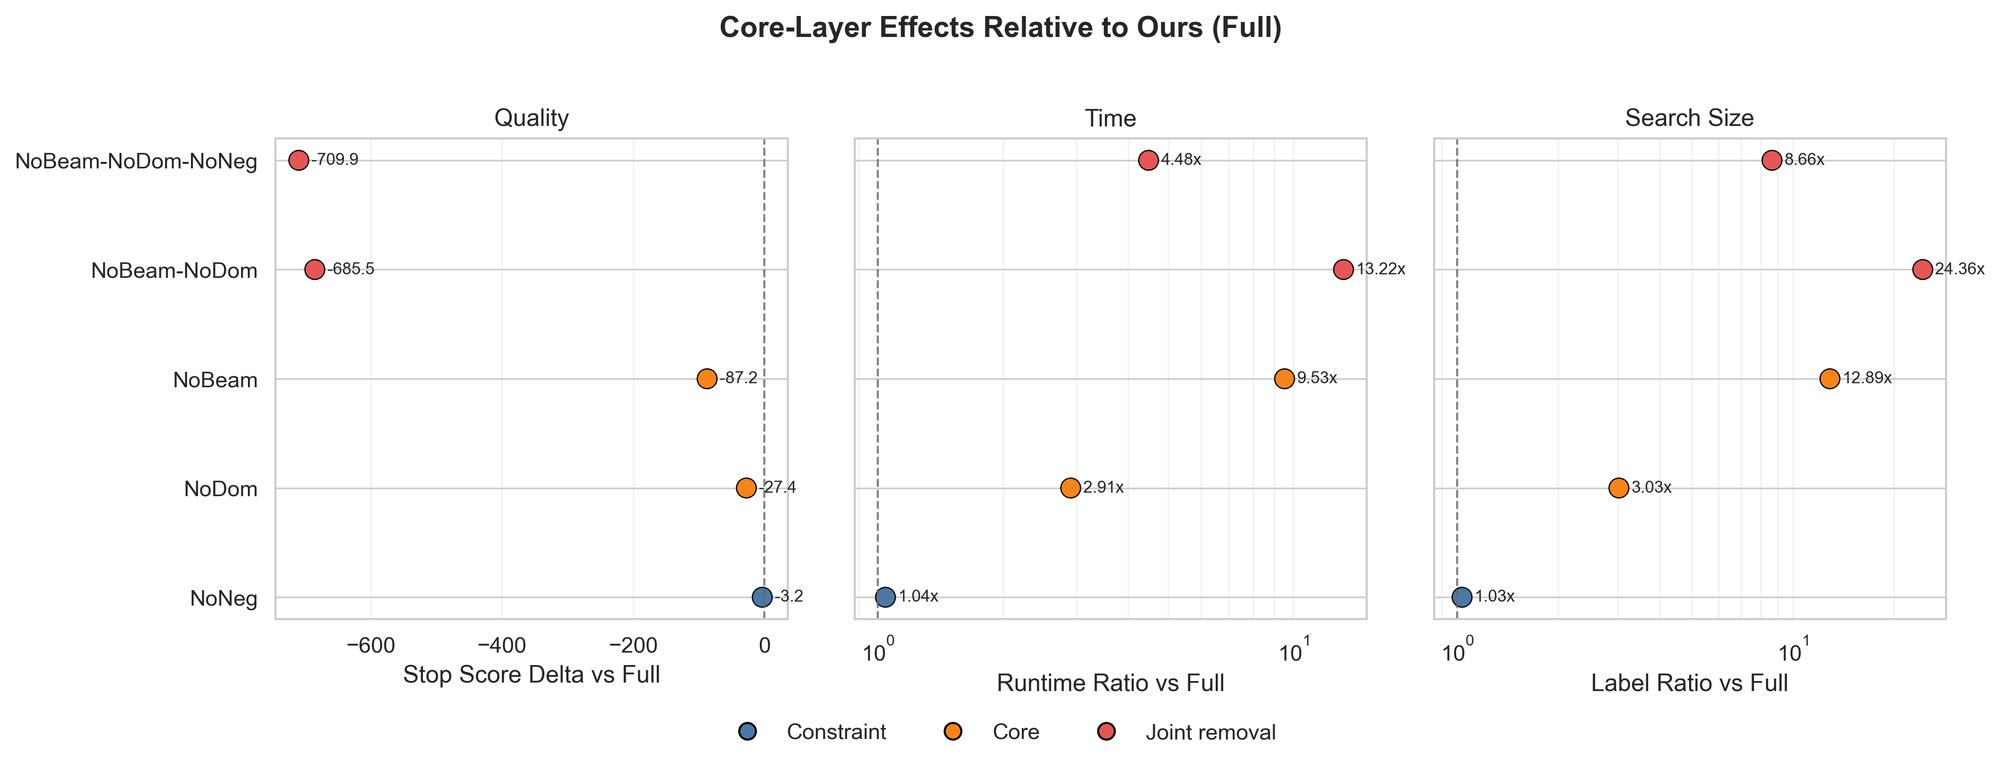
\includegraphics[width=\linewidth]{figures/exp2/exp2_core_layer_delta.pdf}
    \caption{Relative effects of the main ablation variants with respect to \texttt{Ours (Full)}. This figure makes the current interpretation explicit: Beam and Dominance are the two core search-space control layers, while Negative has a role-separated effect.}
    \label{fig:exp2_labels}
\end{figure}

\subsubsection{Supporting Study A: Budget-Sliced View of Beam and Dominance}
To evaluate RQ5, we compare the 4h and 8h slices of the same main ablation.
The point is not that Beam is always beneficial in exactly the same way,
but that its interaction with the budget length is informative.

\begin{table}[t]
    \centering
    \caption{Budget-sliced comparison of \texttt{Full} and \texttt{NoBeam}.}
    \label{tab:exp2_beam_support}
    \resizebox{\columnwidth}{!}{%
        \begin{tabular}{llrrr}
            \toprule
            Budget & Method        & StopScore & Elapsed (ms) & CapHit (\%) \\
            \midrule
            4h     & Ours (Full)   & 737.04    & 771.47       & 0.00        \\
            4h     & Ours (NoBeam) & 803.80    & 27076.50     & 18.89       \\
            \midrule
            8h     & Ours (Full)   & 1261.50   & 8564.82      & 0.00        \\
            8h     & Ours (NoBeam) & 1020.28   & 61897.36     & 100.00      \\
            \bottomrule
        \end{tabular}
    }
\end{table}

Table~\ref{tab:exp2_beam_support} shows a budget-dependent effect.
At 4h, removing Beam can buy some extra score (\(803.80\) vs \(737.04\)),
but only by paying \(35.10\times\) runtime and a nontrivial cap-hit rate.
At 8h, the same relaxation no longer helps: \texttt{Full} dominates
\texttt{NoBeam} on both score and runtime, and \texttt{NoBeam} hits the cap on
all tasks.
Therefore, RQ5 is supported in a more precise form:
Beam is one of the two core search-space control layers, and its importance
becomes especially visible as the budget grows.

\subsubsection{Supporting Study B: Negative Pruning for Theme-Constrained Tasks}
For RQ6, we use the project-aligned route-theme task rather than the old keyword-only
theme benchmark.
The study contains \(384\) paired route-theme cases and compares
\texttt{Full} vs \texttt{NoNeg} under the same starts, departures, and budgets.

\begin{table}[t]
    \centering
    \caption{Supporting route-theme study for Negative pruning.}
    \label{tab:exp2_theme_macro}
    \resizebox{\columnwidth}{!}{%
        \begin{tabular}{lrrrrr}
            \toprule
            Method       & RideMinutes & ThemeScore & ThemeHit & ThemeSat & Elapsed (ms) \\
            \midrule
            Ours (Full)  & 318.98      & 13.81      & 0.965    & 0.958    & 18473.95     \\
            Ours (NoNeg) & 281.09      & 5.58       & 0.677    & 0.646    & 6304.29      \\
            \bottomrule
        \end{tabular}
    }
\end{table}

At the paired-case level, Full improves theme-hit ratio in \(226/384\) pairs,
with only \(2\) regressions, and the final selected route changes in \(366/384\) pairs.
The mean deltas are \(+0.288\) in ThemeHit,
\(+0.313\) in ThemeSat,
\(+37.89\) in RideMinutes,
and \(+12.17\) s in runtime.
This is the intended role of Negative pruning:
it is not the main speedup layer, but it does preserve route-theme fidelity in
the project-style task.
Supplementary visualizations are provided in Appendix A
(Figures~\ref{fig:app_exp2_theme_dumbbell}--\ref{fig:app_exp2_theme_tradeoff}).

\subsubsection{Interpretation: Why the Three Layers Are All Meaningful}
Experiment 2 provides complementary evidence:
\begin{itemize}[leftmargin=1.5em]
    \item \textbf{Dominance pruning} is one of the two core scalability layers; removing it causes a clear search-space blow-up.
    \item \textbf{Beam pruning} is the other core scalability layer; removing it can occasionally buy score at short budgets, but it becomes unstable and expensive as the budget grows.
    \item \textbf{Negative pruning} is a semantic-alignment layer; it improves route-theme preservation, with an explicit runtime trade-off.
\end{itemize}
Therefore, the three-layer design is justified as a \emph{functional decomposition}:
joint search-space control (Beam + Dominance) and objective alignment (Negative).

\subsection{Experiment 3: Balance Analysis Supplementing Experiment 1}
\subsubsection{Objective and Protocol}
Experiment 3 is not another independent benchmark.
Instead, it supplements Experiment 1 by asking whether the methods remain close
to the quality--speed ideal point under the same stop-score task.
The goal is to answer three balance-oriented questions:
\begin{itemize}[leftmargin=1.5em]
    \item \textbf{RQ7 (ideal-point closeness):} Is Ours the method closest to the score--time ideal point?
    \item \textbf{RQ8 (trade-off frequency):} How often is Ours simultaneously higher-score and faster than NSGA-II?
    \item \textbf{RQ9 (budget consistency):} Does the balance advantage hold from 2h to 8h?
\end{itemize}

The current Exp3 analysis is derived from the updated Exp1 source results with
\(10\) origins, \(3\) departure times, \(4\) budgets, and \(5\) stop-score seeds.
This yields \(600\) task-level rows per algorithm and \(120\) base-query rows
after averaging over stop-score seeds.

\subsubsection{Main Balance Results}
The first finding is that Ours is the closest method to the score--time ideal point.
At the task level, Ours has average ideal distance \(0.214\), and at the query level
it further improves to \(0.167\), which is the best among all compared methods.
NSGA-II, despite being the strongest external baseline on raw score, remains much farther
from the ideal point because of its substantially larger runtime.

\begin{table}[t]
    \centering
    \caption{Query-level balance summary of Experiment 3.}
    \label{tab:exp3_balance}
    \resizebox{\linewidth}{!}{%
        \begin{tabular}{lrrrr}
            \toprule
            Method       & Stop Score & Elapsed (ms) & Ideal distance & Avg. balance rank \\
            \midrule
            Ours (Full)  & 826.90     & 4165.67      & 0.1672         & 1.73              \\
            ILS+2opt     & 697.46     & 518.79       & 0.3201         & 2.50              \\
            VNS          & 645.00     & 169.31       & 0.3996         & 3.53              \\
            SA           & 589.46     & 130.80       & 0.5297         & 4.66              \\
            McRAPTOR     & 546.70     & 3684.86      & 0.5489         & 4.63              \\
            NSGA-II      & 760.66     & 27351.18     & 0.6292         & 5.03              \\
            Greedy (L=3) & 416.99     & 3.05         & 0.7975         & 6.41              \\
            Pure RAPTOR  & 320.31     & 56483.31     & 1.2516         & 7.48              \\
            \bottomrule
        \end{tabular}}
\end{table}

Figure~\ref{fig:exp3_main} summarizes the role of Experiment 3 as a balance
analysis supplement to Experiment 1 rather than as a separate claim that Ours
wins every single task.

\begin{figure}[t]
    \centering
    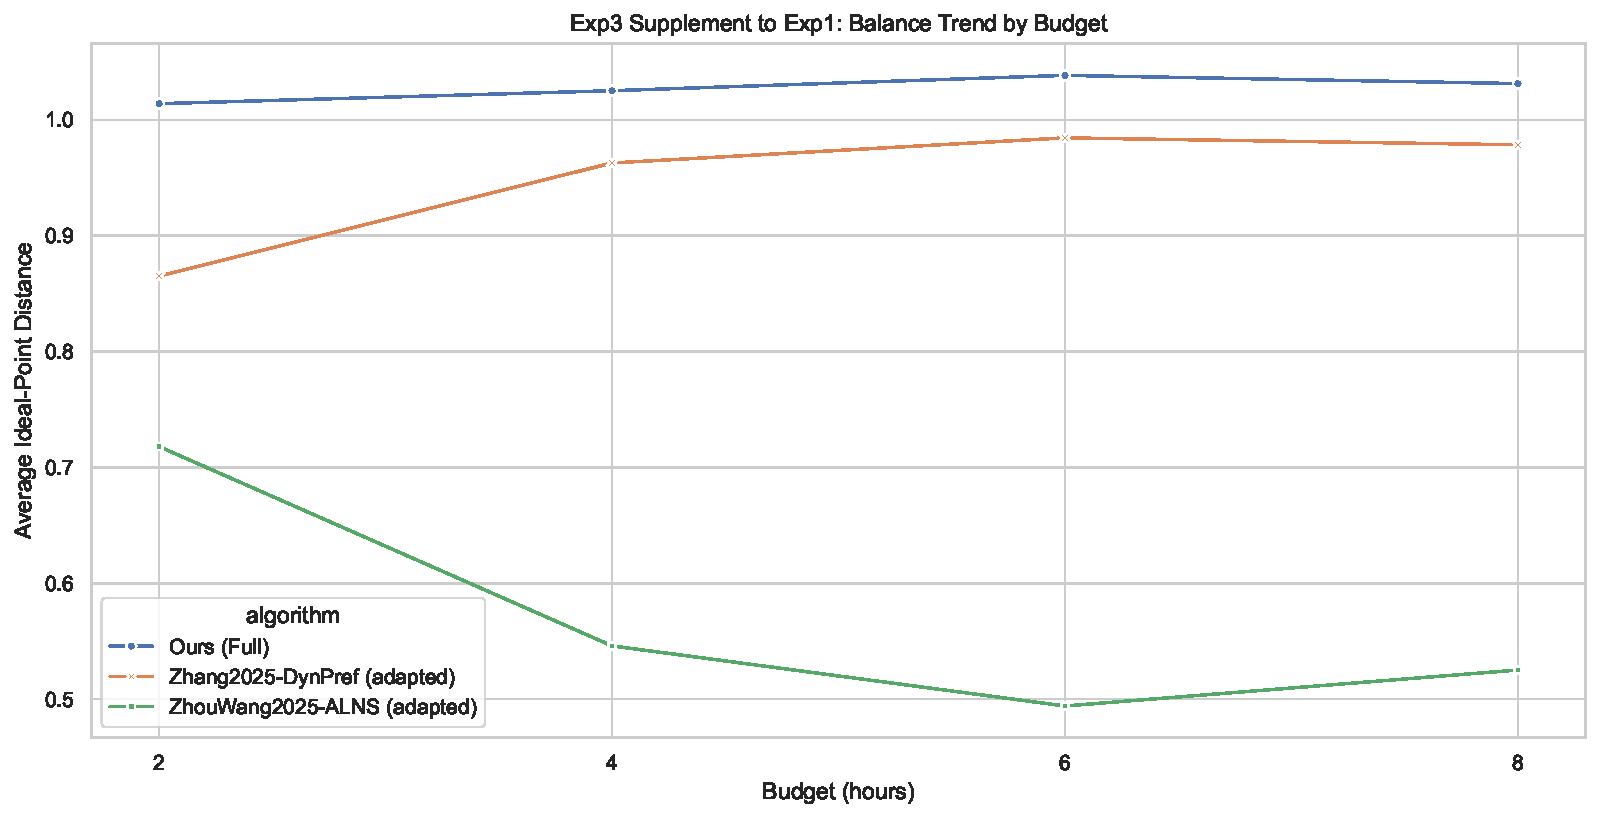
\includegraphics[width=\linewidth]{figures/exp3/exp3_ideal_distance.pdf}
    \caption{Experiment 3 as a balance analysis supplement to Experiment 1. The primary metric is \texttt{ideal\_distance}, shown across the 2h--8h budgets.}
    \label{fig:exp3_main}
\end{figure}

\subsubsection{Budget-Sliced View}
The budget-sliced balance view is also consistent.
At 2h, Ours has ideal distance \(0.2482\) vs \(0.7026\) for NSGA-II.
At 4h, Ours has ideal distance \(0.1097\) vs \(0.5888\) for NSGA-II.
At 6h, Ours has ideal distance \(0.1656\) vs \(0.5963\) for NSGA-II.
At 8h, Ours has ideal distance \(0.3342\) vs \(0.6602\) for NSGA-II.
Thus, the balance advantage is visible throughout the full 2h--8h range,
not only in the previously reported 4h and 8h slices.

\subsubsection{Ours vs NSGA-II Trade-Off Counts}
The second finding is that the ideal-distance advantage is not merely an average effect.
At the task level, Ours is both higher-score and faster than NSGA-II in \(358/600\) tasks.
At the query level, the same pattern holds in \(82/120\) queries.
By budget, the query-level counts are \(17/30\) at 2h, \(27/30\) at 4h,
\(19/30\) at 6h, and \(19/30\) at 8h.

\subsubsection{Interpretation}
Experiment 3 supports three practical claims:
\begin{itemize}[leftmargin=1.5em]
    \item Ours is the closest method to the score--time ideal point under the current Exp1 task;
    \item the Exp1 superiority claim is reinforced by the fact that Ours is simultaneously higher-score and faster on many tasks and queries;
    \item the current balance conclusion is stable across the full 2h--8h budget range, with the clearest lead at 4h and consistent advantage at 6h and 8h.
\end{itemize}
Therefore, Exp3 is best interpreted as a \emph{supplementary balance analysis}
for Experiment 1 rather than as an independent parameter-sensitivity benchmark.

\subsection{Experiment 4: Route Case Study}
\subsubsection{Objective and Positioning}
Experiment 4 is not designed as another benchmark.
Its purpose is to illustrate the quantitative differences observed in Experiments 1 and 3
through concrete route examples, making the results more interpretable.
We address the following questions:
\begin{itemize}[leftmargin=1.5em]
    \item \textbf{RQ10 (success case):} Can the score and speed advantages of Ours be visually confirmed on specific queries?
    \item \textbf{RQ11 (balance case):} Is the quality--speed balance claim reflected in the route structure?
    \item \textbf{RQ12 (limitation):} Are there queries where Ours does not achieve the highest score?
\end{itemize}

\subsubsection{Case Selection Protocol}
To avoid arbitrary cherry-picking, the cases are selected from the Experiment 1 results
using systematic criteria.
We use three cases from the score-guided benchmark:
\begin{itemize}[leftmargin=1.5em]
    \item \textbf{Case A (success):} the query where Ours clearly wins on both stop score and generation time;
    \item \textbf{Case B (balance):} a query where Ours is not the top scorer, but achieves the best quality--speed balance;
    \item \textbf{Case C (counterexample):} a query where Ours is faster but NSGA-II reaches a higher score.
\end{itemize}
Each case compares Ours against NSGA-II and one additional baseline,
with stop score, generation time, score per hour, and scored stops reported per route.

\subsubsection{Main Results}
Table~\ref{tab:exp4_cases} summarizes the three cases.

\begin{table}[t]
    \centering
    \small
    \caption{Route case study: selected cases from Experiment 1.}
    \label{tab:exp4_cases}
    \resizebox{\linewidth}{!}{%
        \begin{tabular}{llrrrr}
            \toprule
            Case & Algorithm & Stop score & Gen time (ms) & Score / hour & Scored stops \\
            \midrule
            A    & Ours      & 1459.0     & 9091.1        & 185.5        & 22           \\
            A    & NSGA-II   & 854.0      & 14129.0       & 108.1        & 13           \\
            A    & VNS       & 508.0      & 37.0          & 68.5         & 10           \\
            \midrule
            B    & Ours      & 1276.0     & 4473.7        & 164.6        & 18           \\
            B    & NSGA-II   & 1590.0     & 18956.2       & 200.8        & 22           \\
            B    & SA        & 1506.0     & 156.4         & 192.7        & 20           \\
            \midrule
            C    & Ours      & 1358.0     & 2730.8        & 187.3        & 18           \\
            C    & NSGA-II   & 1556.0     & 20367.1       & 207.9        & 19           \\
            C    & VNS       & 1461.0     & 192.6         & 186.5        & 19           \\
            \bottomrule
        \end{tabular}}
\end{table}

Case A is the clearest success example.
Ours achieves a stop score of 1459.0 with a generation time of 9091.1 ms,
while NSGA-II reaches only 854.0 in 14129.0 ms.
This confirms that there exist queries where Ours simultaneously
achieves a substantially higher score and a shorter generation time.

Case B is the intended quality--speed balance example.
Here Ours does not achieve the highest score (1276.0 vs 1590.0 for NSGA-II),
but its generation time is much shorter (4473.7 ms vs 18956.2 ms).
This case visually reinforces the Experiment 3 claim
that Ours most often stays close to the score--time ideal point.
Figure~\ref{fig:exp4_main} visualizes the main route-level contrast between the
success case and the balance case.

\begin{figure}[t]
    \centering
    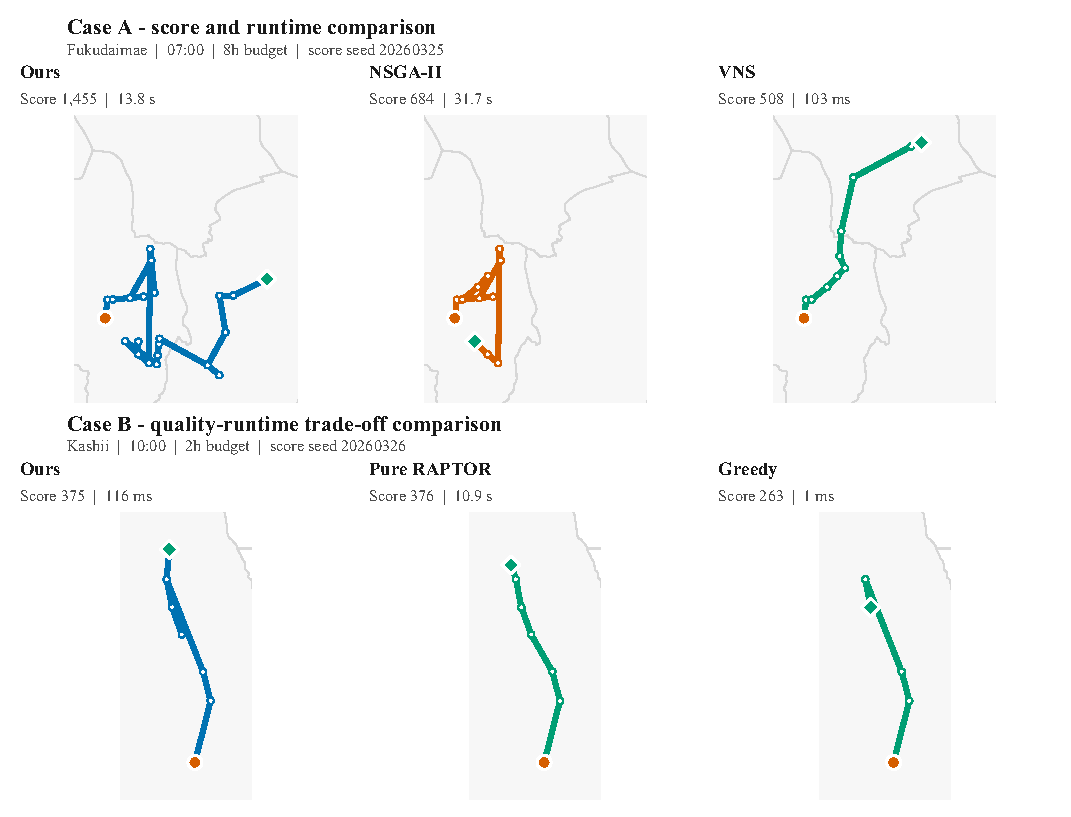
\includegraphics[width=\linewidth]{figures/exp4/exp4_main_cases.pdf}
    \caption{Route case study main panels. Top: Case A, where Ours clearly leads in both stop score and generation time. Bottom: Case B, where Ours is not the top scorer but achieves the best quality--speed balance.}
    \label{fig:exp4_main}
\end{figure}

Case C is kept as a counterexample.
Ours is faster (2730.8 ms vs 20367.1 ms) but does not reach the highest score
(1358.0 vs 1556.0 for NSGA-II).
This case is placed in Appendix A (Figure~\ref{fig:app_exp4_appendix})
to explicitly avoid claiming that Ours wins on every query.

\subsubsection{Interpretation}
Experiment 4 provides a route-level interpretability check for the aggregate
findings.
Case A and Case B visually confirm the quantitative claims of Experiments 1 and 3,
while Case C improves credibility by showing a limitation.

\section{Discussion}
The experimental results support a more precise claim than simply
``ReRAPTOR obtains the best routes.''
Under the current seeded stop-reward benchmark, the main advantage of
ReRAPTOR is that it most consistently balances route quality and computation
time.
In Experiment~1, it achieves the highest overall average stop score and
outperforms NSGA-II by \(+8.71\%\) on that metric while remaining
\(6.57\times\) faster on average.
Experiment~3 strengthens this interpretation: ReRAPTOR has the best
query-level ideal distance (\(0.1672\)) and is simultaneously higher-score and
faster than NSGA-II in \(82/120\) base queries.
At the same time, the case study in Experiment~4 makes clear that the method is
not universally dominant on every individual query, which is important for a
credible evaluation.

The ablation results also clarify how the proposed method should be understood.
Beam pruning and Dominance pruning are not optional implementation details; they
are the two main mechanisms that keep the label search computationally
manageable.
When Dominance is removed, runtime and label count increase substantially even
though the search still finishes.
When Beam is removed, the search becomes much more expensive, and the effect is
especially severe for the 8-hour budget where cap hits occur in all tasks.
When both are removed together, the search space grows too quickly and route
quality also degrades.
Negative pruning plays a different role.
It does not provide the main speedup on the generic stop-reward benchmark, but
the theme-constrained supporting study shows that it improves theme-hit ratio
and route-theme satisfaction, so its value lies in objective alignment rather
than raw scalability.

These findings have two practical implications.
First, a timetable-feasible transit itinerary planner does not need to maximize
score at any computational cost to be useful; for interactive or repeated query
settings, the quality--speed balance is often the more relevant criterion.
Second, the objective module should remain explicit.
The same search backbone behaves differently depending on whether the task
rewards geometry, stop collection, or thematic coherence, and the experiments
show that the pruning layers interact with those objectives in different ways.
This argues against treating all value-maximizing transit planning tasks as
instances of a single fixed scalar objective.

Several limitations remain.
The experiments are based on one city's Ekispert-provided transit schedule
data, so cross-city generalization is not yet established.
The main benchmark uses seeded stop rewards as a synthetic proxy for
value, which is useful for controlled comparison but is still not a substitute
for user studies or real preference learning.
In addition, some implementation constants, such as beam width, lookahead
window, and timeout-related guards, are fixed practical defaults rather than
globally optimized settings.
Future work should therefore study transfer across cities, learn reward modules
from observed user behavior, and investigate adaptive pruning policies that vary
with budget length and search difficulty.

\section{Conclusion}
This paper presented ReRAP\-TOR, a reverse-objective RAPTOR-style method for
time-budgeted value-maximizing transit itinerary planning on timetable-based
transit schedules. Its main methodological contribution is to optimize route
value during timetable-feasible expansion through a shared search backbone with
pluggable objective modules and a three-layer pruning design, rather than
scoring candidate routes only after they are fully constructed.

Across the main stop-reward benchmark, ReRAPTOR achieves the best overall
quality--speed profile among the compared baselines.
It attains the highest average stop score (\(826.90\)), exceeds NSGA-II by
\(8.71\%\) on that metric, and remains \(6.57\times\) faster on average.
The supplementary balance analysis shows that it is also the closest method to
the score--time ideal point, and the ablation study shows that Beam and
Dominance are the two core scalability layers, whereas Negative pruning mainly
improves semantic alignment in constrained theme tasks.
The route case study further confirms both the strengths of the method and the
fact that it does not win every query.

Overall, the results indicate that ReRAPTOR is a practical approach for
value-oriented transit itinerary planning when the goal is not only to obtain
high-scoring routes, but to do so with stable and usable response times.
This makes it a strong foundation for future work on preference-aware,
theme-aware, and city-scale transit exploration systems.

\section*{Acknowledgment}
This study used transit schedule data for Fukuoka provided through Ekispert
services (\begin{CJK*}{UTF8}{min}Powered by Ekispert API\end{CJK*}).

\bibliographystyle{spmpsci}
\bibliography{references_draft}

\appendix
\section{Appendix A: Supplementary Visualizations (Exp1--Exp4)}
This appendix collects the supplementary figures referenced in the main text.
Their purpose is to make the main claims more transparent rather than to add a
new evaluation story.
Appendix figures for Experiment~1 show robustness across random stop-score
seeds, those for Experiment~2 visualize the trade-offs behind the ablation and
theme-support studies, the Experiment~3 figure complements the ideal-distance
summary with a quality--speed scatter view, and the Experiment~4 appendix keeps
an explicit counterexample to avoid overclaiming.

\subsection{Experiment 1 Supplementary Figures}
The figure in this subsection reports seed-level stability for the updated
seeded stop-reward benchmark.
It supports the main-text statement that the advantage of ReRAPTOR over
NSGA-II remains positive across the tested score seeds, even though the gap
varies by seed and budget.

\begin{figure}[t]
    \centering
    \includegraphics[width=\linewidth]{figures/exp1/exp1_score_guided_multiseed_seed_stability_2h4h6h8h.pdf}
    \caption{Supplementary to Experiment 1: score-seed stability under the seeded stop-reward benchmark.}
    \label{fig:app_exp1_seed}
\end{figure}

\subsection{Experiment 2 Supplementary Figures}
These figures provide additional evidence for the role separation observed in
the ablation study.
The Pareto-style scatter highlights the efficiency frontier of the core pruning
variants, while the remaining figures summarize how Negative pruning changes
route-theme behavior in the supporting study at the aggregate level.

\begin{figure}[t]
    \centering
    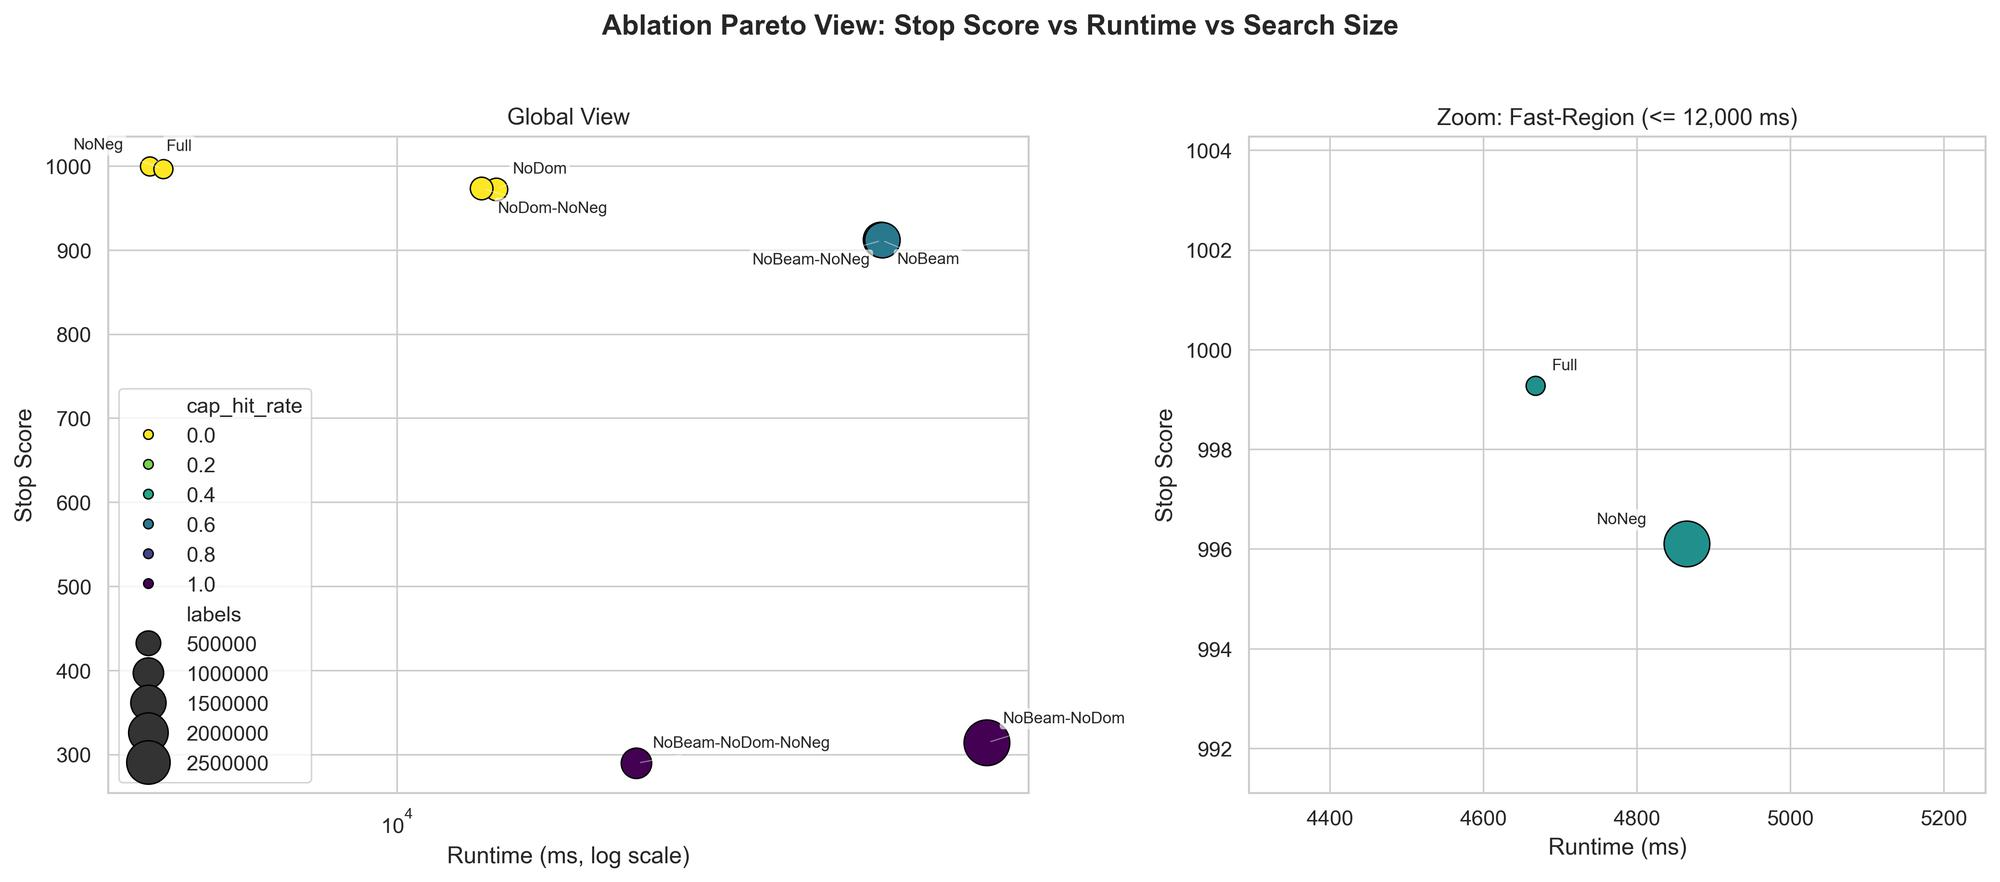
\includegraphics[width=\linewidth]{figures/exp2/exp2_ablation_pareto_scatter.pdf}
    \caption{Supplementary to Experiment 2: Pareto-style ablation scatter view.}
    \label{fig:app_exp2_pareto}
\end{figure}

\begin{figure}[t]
    \centering
    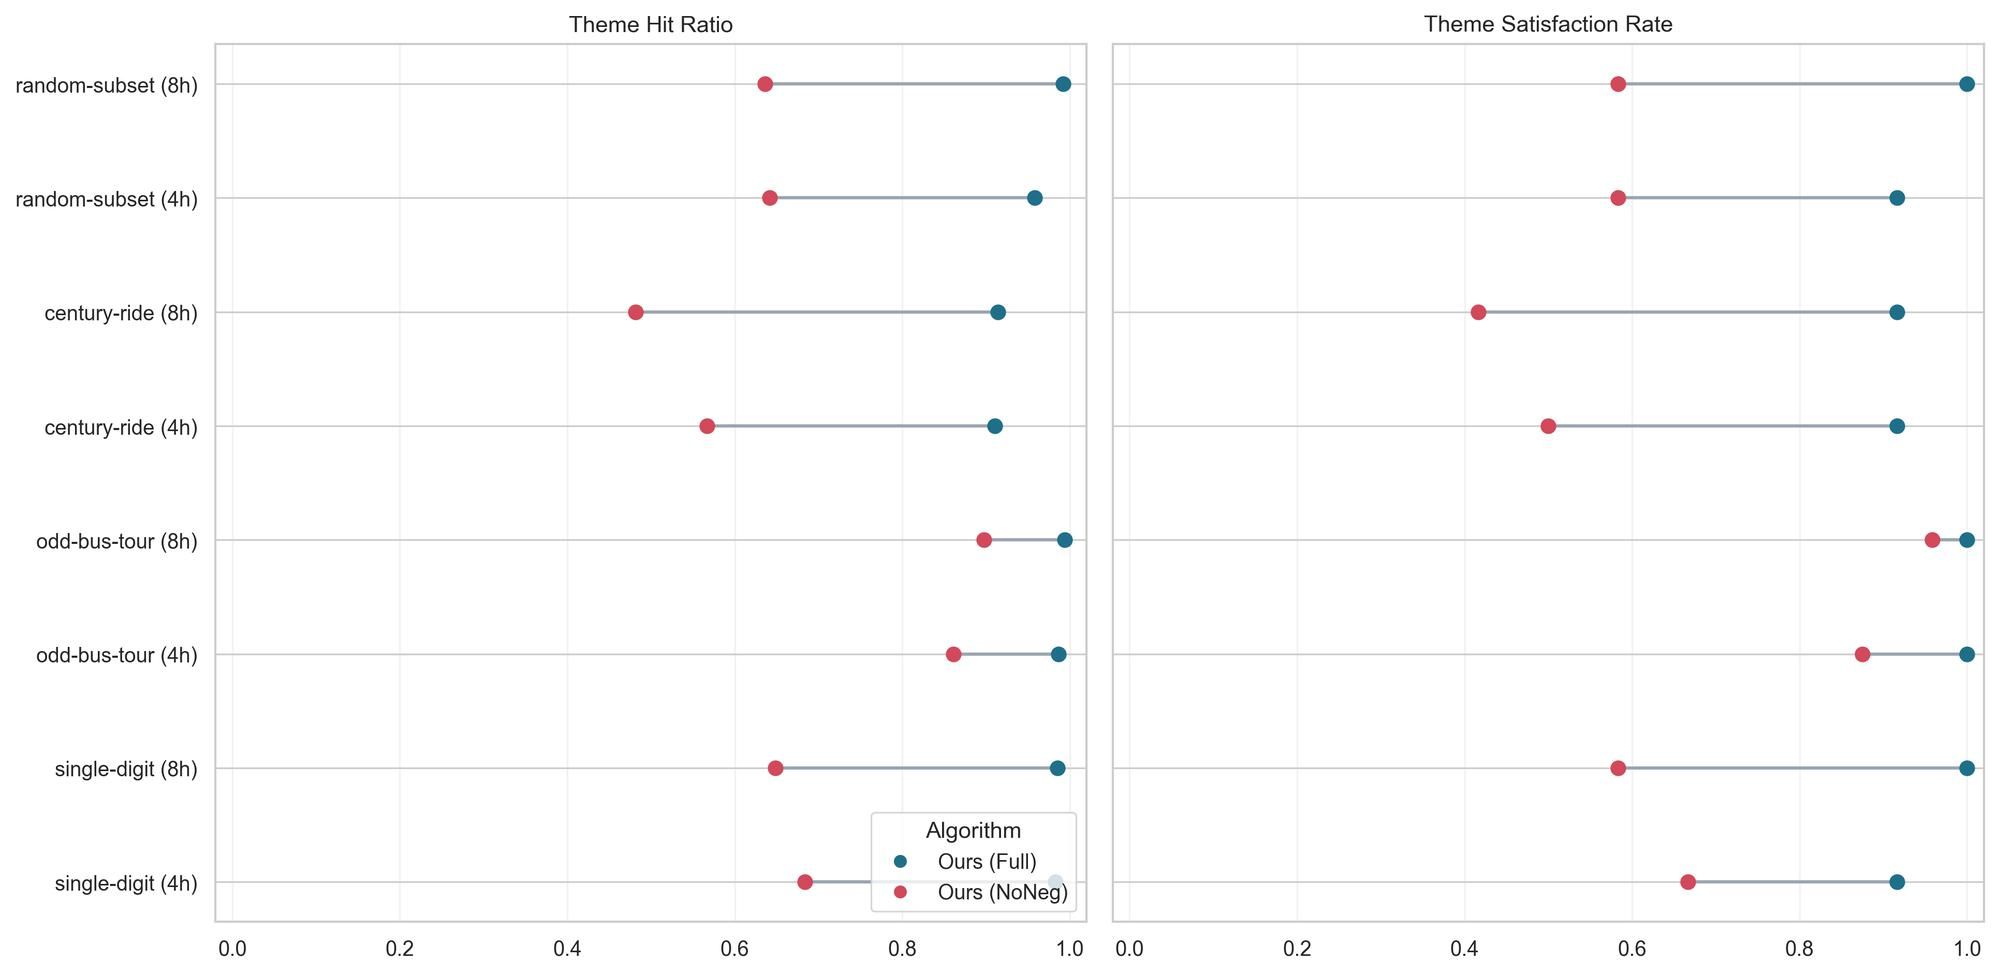
\includegraphics[width=\linewidth]{figures/exp2/exp2_supporting_theme_dumbbell.pdf}
    \caption{Supplementary to Experiment 2: paired route-theme gains of \texttt{Full} over \texttt{NoNeg}.}
    \label{fig:app_exp2_theme_dumbbell}
\end{figure}

\begin{figure}[t]
    \centering
    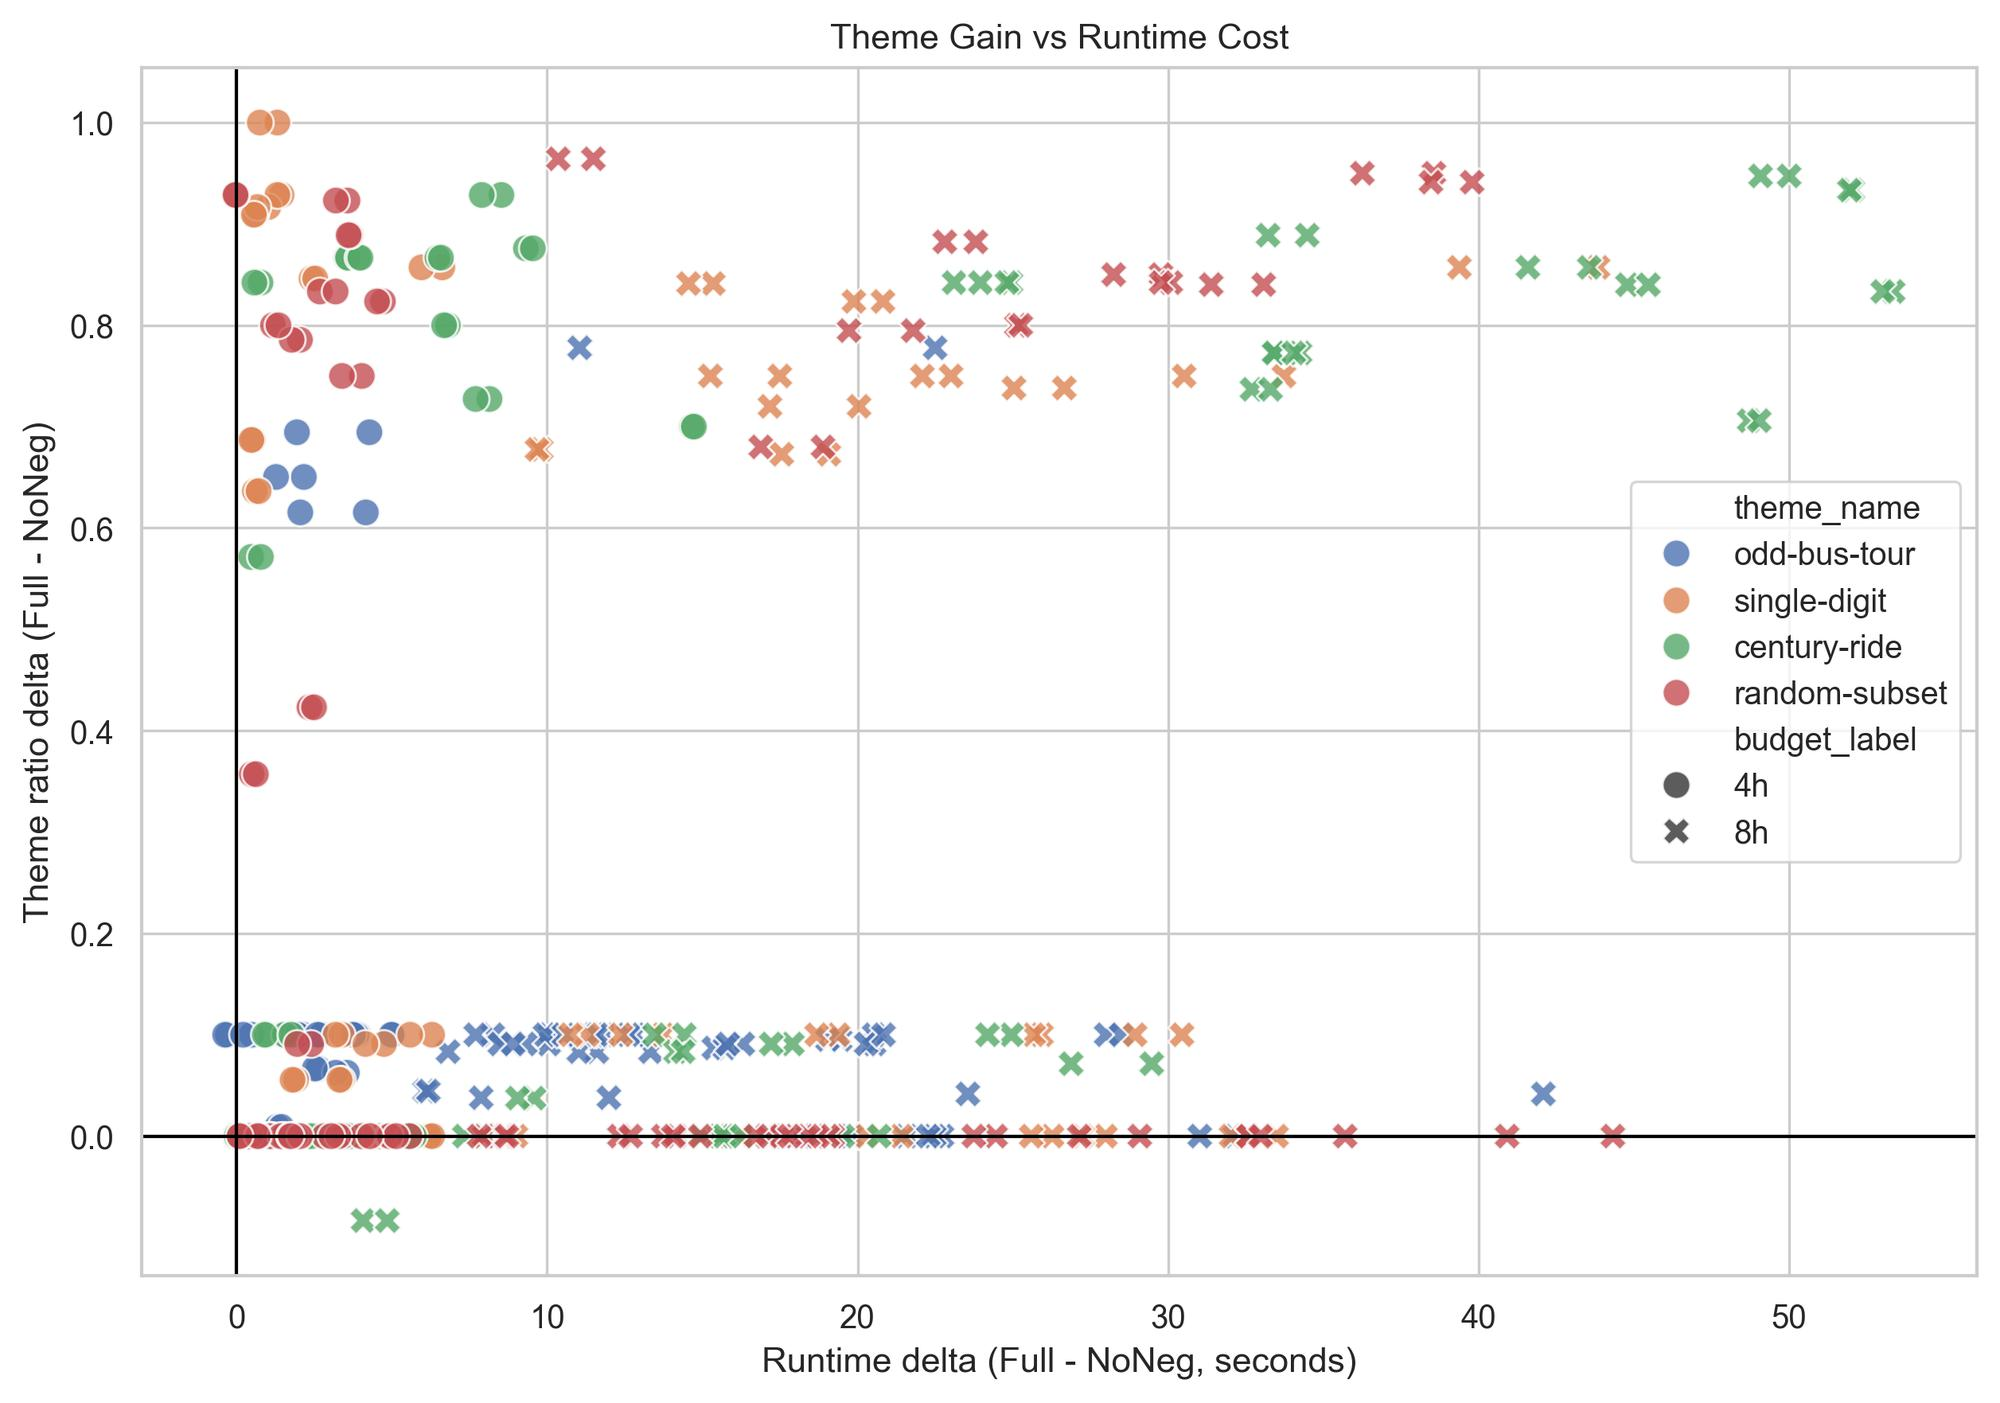
\includegraphics[width=\linewidth]{figures/exp2/exp2_supporting_negative_tradeoff.pdf}
    \caption{Supplementary to Experiment 2: trade-off view of route-theme preservation and runtime overhead.}
    \label{fig:app_exp2_theme_tradeoff}
\end{figure}

\subsection{Experiment 3 Supplementary Figures}
The following scatter plot complements the main ideal-distance figure by showing
how the methods are distributed in the quality--speed plane.
It helps explain why ReRAPTOR is closest to the ideal point even though some
baselines are occasionally faster or occasionally higher-scoring on individual
queries. Figure~\ref{fig:app_exp3_scatter} provides this supplementary
quality--speed view.

\begin{figure}[t]
    \centering
    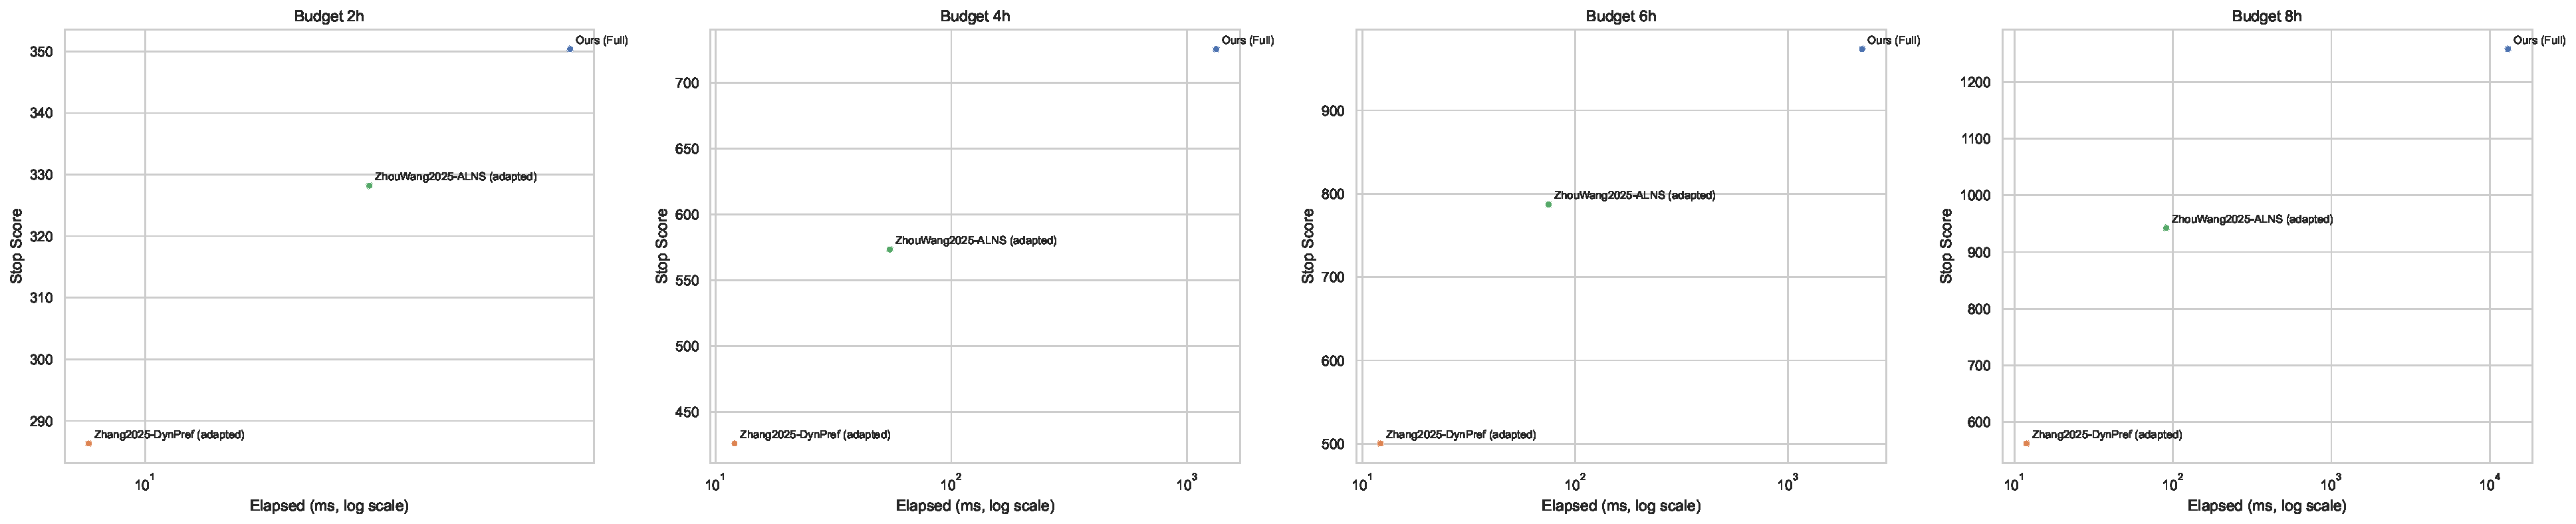
\includegraphics[width=\linewidth]{figures/exp3/exp3_quality_speed_scatter.pdf}
    \caption{Supplementary to Experiment 3: quality--speed scatter around the ideal-point balance view.}
    \label{fig:app_exp3_scatter}
\end{figure}

\subsection{Experiment 4 Supplementary Figures}
The appendix case for Experiment~4 is intentionally retained as a limitation
example.
It shows a query where ReRAPTOR is substantially faster than NSGA-II but does
not achieve the highest stop score, reinforcing that the contribution of the
method is overall balance rather than universal per-query dominance.
Figure~\ref{fig:app_exp4_appendix} shows this explicit counterexample.

\begin{figure}[t]
    \centering
    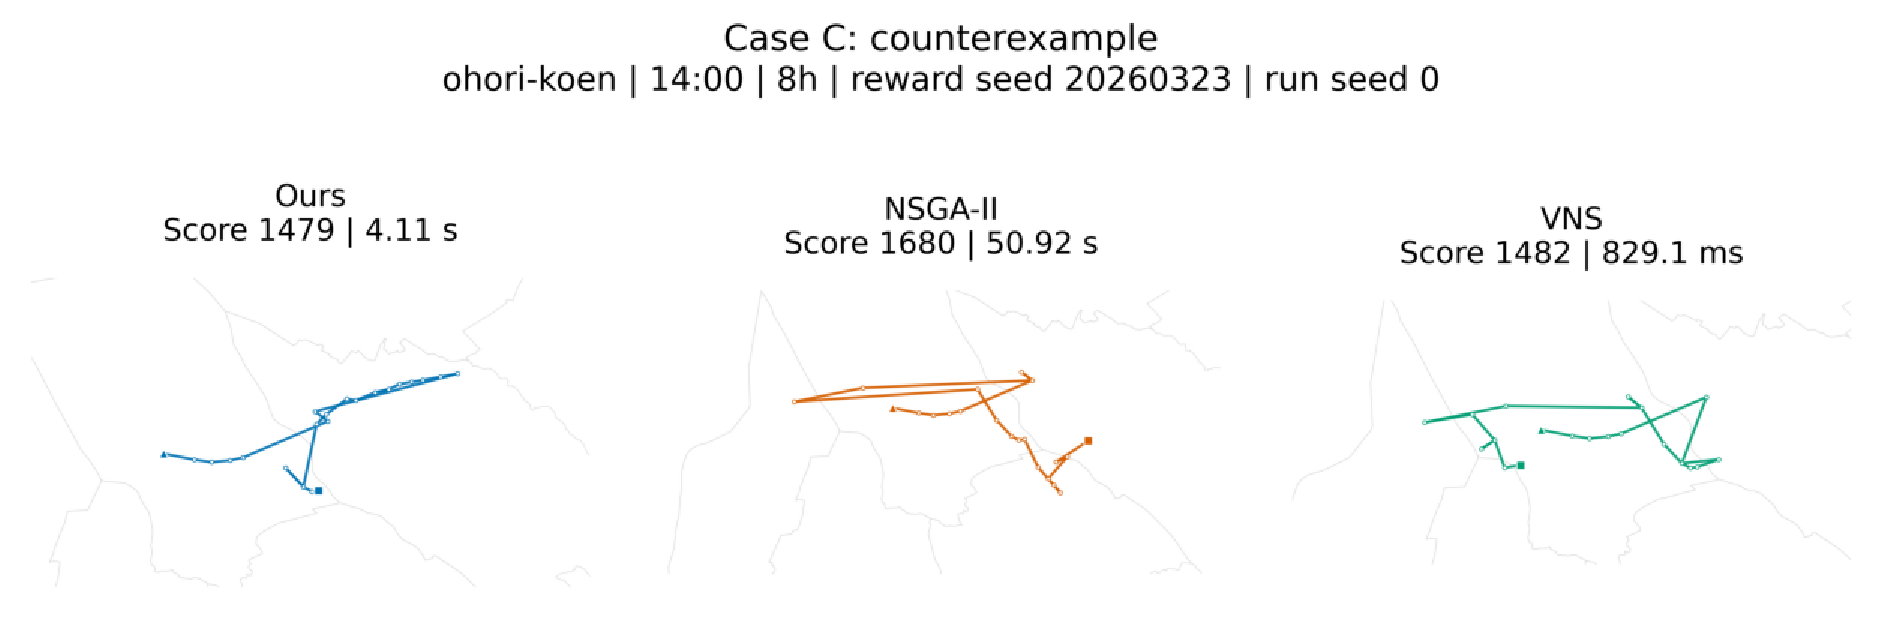
\includegraphics[width=\linewidth]{figures/exp4/exp4_appendix_cases.pdf}
    \caption{Supplementary to Experiment 4: Case C, kept as a counterexample where Ours is faster but does not reach the highest stop score.}
    \label{fig:app_exp4_appendix}
\end{figure}

\end{document}
% end of file template.tex
